\documentclass[conference]{IEEEtran}
\IEEEoverridecommandlockouts
% The preceding line is only needed to identify funding in the first footnote. If that is unneeded, please comment it out.
\usepackage{cite}
\usepackage{amsmath,amssymb,amsfonts}
\usepackage{algorithmic}
\usepackage{graphicx}
\usepackage{textcomp}
\usepackage{xcolor}
\usepackage{subcaption}
\usepackage{cuted}
\usepackage{mathtools}
\usepackage{booktabs}

\def\BibTeX{{\rm B\kern-.05em{\sc i\kern-.025em b}\kern-.08em
    T\kern-.1667em\lower.7ex\hbox{E}\kern-.125emX}}
\begin{document}

\title{Image Based Visual Servoing for Landmine Detection using Quadrotors\\
% {\footnotesize \textsuperscript{*}Note: Sub-titles are not captured in Xplore and
% should not be used}
\thanks{This study is conducted in a Ph.D. project, funded by the Mexican Consejo Nacional de Ciencia y Tecnología (CONACyT) and Cranfield University.}
}

\author{\IEEEauthorblockN{1\textsuperscript{st} Alejandro Dena}
\IEEEauthorblockA{%\textit{Centre for Electronic Warfare, Information and Cyber} \\
\textit{Cranfield University}\\
% Defence Academy of the United Kingdom, Shrivenham, SN6~8LA, UK.\\
j.a.dena-ruiz@cranfield.ac.uk}
\and
\IEEEauthorblockN{2\textsuperscript{nd} Kenan Ahiska}
\IEEEauthorblockA{%\textit{Centre for Electronic Warfare, Information and Cyber} \\
\textit{Cranfield University}\\
% Defence Academy of the United Kingdom, Shrivenham, SN6~8LA, UK.\\
kenanahiska@gmail.com}
\and
\IEEEauthorblockN{3\textsuperscript{rd} Nabil Aouf}
\IEEEauthorblockA{%\textit{ Department of Electrical and Electronic Engineering} \\
\textit{City University of London, UK}\\
% Northampton Square, London, EC1V~0HB, UK\\
nabil.aouf@city.ac.uk}
}

\maketitle

\begin{abstract}
This paper presents a technical approach for landmine detection with quadrotors using image based visual servoing (IBVS) on thermal images. Considering the difference in temperature between the ground soil and possible buried targets, thermal images are used to estimate target position in an unscented Kalman filter framework: accelerometers, gyroscopes and GPS measurements are integrated in loosely coupled manner as the navigation solution. At first, the quadrotor quipped with single thermal camera estimates the target's depth by following a special ellipsoid trajectory and then using IBVS, it approaches to the target up to one meter distance. In order to control the drone to flight close to the ground, a ground effect compensated controller is also considered in the implementation. Results show that for landmine detection purposes using IBVS on thermal images, with ground effect compensated control, an overall error around 20 pixels is achievable. 
\end{abstract}

\begin{IEEEkeywords}
Quadrotor, IBVS, visual servoing, ground effect, thermal imaging, landmine detection
\end{IEEEkeywords}

\section{Introduction} Detection of landmines is gaining more interest from the public and private institutions, universities and industry \cite{ICBL2018}. The latest advances in technology are offering newer solutions and new detection techniques. One of the most focused approaches is the use of aerial vehicles to perform landmine detection and detonation, allowing the user to perform the operations remotely, otherwise the vehicles are autonomous. The main disadvantage of these aerial vehicles is their limited payload and flight time, which necessitates design of advanced control techniques.

Visible cameras mounted on quadrotors to perform object detection and tracking have been extensively used over the last decade. Azrad et al. showed an example of object tracking using a color detection algorithm on visible spectrum images, from a camera pointing downwards \cite{AZRAD2010}. The authors used PID controllers performed visual servoing for a designated target on the floor. 

Similar to image-based visual servoing (IBVS), but using the points detected on a particular object is presented by Popova et al. on simulation results \cite{Popova}. Among the experimental studies on visual servoing for quadrotors, Ho et al. performed experiments with a known target on the floor and a visible camera pointing downwards mounted on the quadrotor together with an ultrasonic sensor for estimating the target depth \cite{Ho2013}. Pose estimation was achieved by implementing a Kalman filter to fuse these sensors with inertial measurements for the velocity generation process of IBVS. Lee et al. showed some experimental results of a quadrotor performing IBVS to a known marker, where the depth is obtained based on the previous knowledge of the dimensions of the marker \cite{Lee2011}. Similarly, among IBVS studies for target detection and tracking for a moving platform setups, Falanga et al. used the known physical distance between the points on the image place and the real dimension of the marker \cite{Falanga2017}, while Sani et al. benefitted from Kalman filter framework for sensor fusion \cite{Sani2019}.

In the literature, simulation and experimental results for testing different linear and non-linear control laws integrated with the IBVS are available in [\cite{Zheng2018}, \cite{Jabbari2012} and \cite{Bourquardez2009}], and Araar et al. showed the implementation of IBVS on a quadrotor performing power line inspection where they conducted their experiments in an constrained indoor environment equipped with the OptiTrack camera motion system \cite{Araar2014}. Similarly King used the same setup for a quadrotor applying IBVS to land on a moving platform \cite{King2017}. 

Rodriguez et al. developed a software ROS package to work with a quadrotor parrot. They used the onboard visible cameras and controlled the drone manually with a joystick. Thereafter they collected pictures from an field with cans emulating the landmines, with the purpose of proof the possibility of landmine detection. The results showed the applicability of the OpenCV algorithms for post processing of the images, the detection and classification of the target objects \cite{Rodriguez2014}. Nikulin et al. proposed the use of a quadrotor and a thermal camera for detection of small butterfly landmines lying on the ground in their experiments performed on a field using real casings of this explosives. The recorded images are stored for further analysis, where the thermal differences between the ground and the exposed landmines made it possible for distinguish the landmine \cite{Nikulin2018}. Similarly Makki et al. analysed the feasibility of landmine detection using hyperspectral imaging. An extensive set of experiments in the detection area were performed for an hexacopter or octocopter \cite{Makki2018}.

In this work, a solution for landmine detection is proposed, it is based on the use of IBVS on IR images and experimental validation is performed on a quadrotor Pelican. The quadrotor is autonomously controlled using the methods proposed in our previous work in \cite{DenaRuiz2017_1}. The drone uses an onboard computer and the OpenCV libraries to process the thermal images in real-time. The methods assume that there exist differences in temperatures of the ground areas with and without a buried landmine. Accordingly, possible buried target can be spotted as blobs on the thermal images, these blobs are tracked for target location as explained in our previous work in \cite{DenaRuiz2017_2}. After the buried object is localized in 3D with respect to the quadrotor, IBVS is utilized to approach the area where the possible target is buried. Incorporated with IBVS, a ground effect compensating controller design explained in \cite{DenaRuiz2019_1} is considered. 

\section{Modelling and control of quadrotors}
\subsection{Mathematical modelling}
A mathematical model for quadrotors is defined based on Newton-Euler equations, \cite{DenaRuiz2017_1}. In order to eliminate unnecessary complexity, the quadrotor is assumed to be symmetric and rigid. The reference frames and key variables are presented in Fig. \ref{quad_frames}, where $\mathcal{F}_{I}$ represents the inertial frame fixed at a point on the ground and with its $z$ axis pointing upwards, the $x$ and $y$ axes can be chosen following the right hand convention. $\mathcal{F}_{B}$ represents the body frame, with its initial coordinate axes aligned with $\mathcal{F}_{I}$ and its origin is at the center of gravity of the quadrotor, which is assumed to coincide with its geometric centre. Also each propeller have a rotational velocity $\Omega_{i}$ with $i=1:4$, $\Omega_{1}$ and $\Omega_{2}$ are in counter-clockwise direction, whilst $\Omega_{3}$ and $\Omega_{4}$ are in the clockwise direction.

\begin{figure}
    \centering
    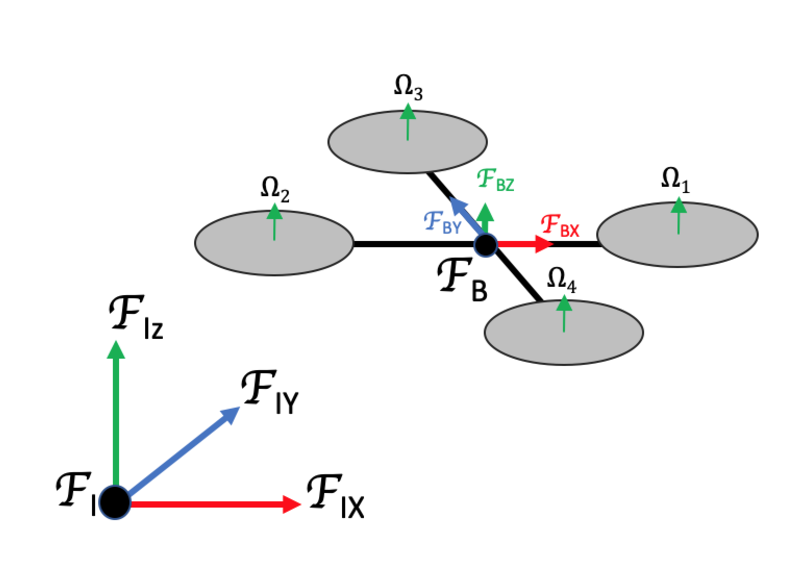
\includegraphics[width=8.5cm, height=6cm]{Images/quad_frames.eps}
    \caption{Body and Inertial frames.}
    \label{quad_frames}
\end{figure}


\begin{align}
    \ddot{X}      &= (\cos\phi\sin\theta\cos\psi + \sin\phi\sin\psi)\frac{1}{m}U_{1} \label{model_1}\\
    \ddot{Y}      &= (\cos\phi\sin\theta\sin\psi - \sin\phi\cos\psi)\frac{1}{m}U_{1}  \label{model_2}\\
    \ddot{Z}      &= (\cos\phi\cos\theta)\frac{1}{m}U_{1}GE - g \label{model_3}\\ 
    \ddot{\phi}   &= \dot{\theta}\dot{\psi}(\frac{I_{yy}-I_{zz}}{I_{xx}})-\frac{J_{r}}{I_{xx}}\dot{\theta}\Omega+\frac{U_{2}}{I_{xx}} \label{model_4}\\
    \ddot{\theta} &= \dot{\phi}\dot{\psi}(\frac{I_{zz}-I_{xx}}{I_{yy}})+\frac{J_{r}}{I_{yy}}\dot{\phi}\Omega+\frac{U_{3}}{I_{yy}} \label{model_5}\\
    \ddot{\psi}   &= \dot{\phi}\dot{\theta}(\frac{I_{xx}-I_{yy}}{I_{zz}})+\frac{U_{4}}{I_{zz}} \label{model_6}
\end{align}

Using Newton's laws of mechanics and Euler's dynamics, the model consists of six equations for the system dynamics and four equations to describe the inputs, as shown in \eqref{model_1}-\eqref{model_6}, where $m$ is the total quadrotor mass, GE represents the ground effect force, \eqref{model_1} - \eqref{model_3} describe the linear accelerations defined in the $\mathcal{F}_{I}$, while \eqref{model_4} - \eqref{model_6} represent the angular accelerations about the centre of gravity of the vehicle in $\mathcal{F}_{B}$. $l$ corresponds to the arm length holding the propeller, $\phi$, $\theta$ and $\psi$ represent the Euler angles. $I_{xx}$, $I_{yy}$ and $I_{zz}$ are the body inertial components, and $J_{r}$ and $\Omega$ are the rotor inertia and rotor speed, respectively. $U_{1}$, $U_{2}$, $U_{3}$ and $U_{4}$ represent the control inputs, as well as total force provided by the four rotors, and the torques in each of the rotation axis. These last four variables will be the system inputs, and are related to the propeller speeds as follow: 

\begin{align}  
U_{1}  &= b(\Omega_{1}^{2} + \Omega_{2}^{2} + \Omega_{3}^{2} + \Omega_{4}^{2}) \label{model_7}\\ 
U_{2}  &= b(\Omega_{3}^{2} + \Omega_{4}^{2}) \label{model_8} \\
U_{3}  &= b(\Omega_{2}^{2} + \Omega_{1}^{2}) \label{model_9} \\
U_{4}  &= d(\Omega_{1}^{2} + \Omega_{2}^{2} - \Omega_{3}^{2} - \Omega_{4}^{2}) \label{model_10} \\
\Omega &= \Omega_{1}^{2} + \Omega_{2}^{2} + \Omega_{3}^{2} + \Omega_{4}^{2} \label{model_11}
\end{align}

\subsection{Ground effect}
It is well known that aerial vehicles with rotors tend to experience some aerodynamic effects as they fly close to surfaces or objects. The aerodynamic effect produced by the interaction between the ground surface and the aerial vehicles is called \textit{ground effect} and it alters the total vehicle thrust. For the case of multirotors, the ground effect becomes complex due to the aerodynamic interaction between a rotor and its neighboring rotors. Among the different models in the literature, the model presented in \cite{DenaRuiz2019_1} is the one that is used in this work. Here the model is based on the method of images and depends on the physical properties of the quadrotor as well as the type of surface, in which the vehicle is hovering.

% \begin{align}
%   GE(z,r,s) = \frac{1}{\splitfrac{1 - (\frac{R}{4z})^{2} - R^{2}(\frac{z}{\sqrt{(d^{2}+4z^{2})^{3}}})} {\splitfrac{- (\frac{R^{2}}{2})(\frac{z}{\sqrt{(2d^{2}+4z^{2})^{3}}}) - 2R^{2}(\frac{z}{\sqrt{(b^{2}+4z^{2})^{3}}}k_{b})}{- 2R^{2}(\frac{z}{\sqrt{(b^{2}+4z^{2})^{3}}}k_{s})}}} \label{dena_ge}
% \end{align}

\begin{strip}
\begin{equation}
    GE(z,r,s) = \frac{1}{1 - (\frac{R}{4z})^{2} - R^{2}(\frac{z}{\sqrt{(d^{2}+4z^{2})^{3}}}) - (\frac{R^{2}}{2})(\frac{z}{\sqrt{(2d^{2}+4z^{2})^{3}}}) - 2R^{2}(\frac{z}{\sqrt{(b^{2}+4z^{2})^{3}}}k_{b}) - 2R^{2}(\frac{z}{\sqrt{(b^{2}+4z^{2})^{3}}}k_{s})} \label{dena_ge}
\end{equation}
\end{strip}

\subsection{Quadrotor control with ground effect compensation}
The quadrotor control is performed according to the work done in \cite{DenaRuiz2017_1}, where the attitude of the vehicle is desired to be near the hovering position, 3 PD controllers are developed for the orientation control in the inner loop, whereas for the drone position is controlled by another 3 PD controllers in cascade. In \eqref{pid_r1} - \eqref{control_3}, $r_{1}$ is the altitude PD controller and $U_{1-4}$ are the inputs of the system.

\begin{align}
r_{1} &= K_{pz}(d_{Z} - Z) + K_{dz} (d_{\dot{Z}} - \dot{Z}) \label{pid_r1}\\
U_{1} &= \frac{m(g+r_{1})}{\cos\phi\cos\theta GE(z,r,s)} \label{thrust_force}\\
U_{2} &= K_{p\phi}(d_{\phi} - \phi) + K_{d\phi} (d_{\dot{\phi}} - \dot{\phi}) \label{control_1}\\
U_{3} &= K_{p\theta}(d_{\theta} - \theta) + K_{d\theta} (d_{\dot{\theta}} - \dot{\theta}) \label{control_2}\\
U_{4} &= K_{p\psi}(d_{\psi} - \psi) + K_{d\psi} (d_{\dot{\psi}} - \dot{\psi}) \label{control_3} 
\end{align}

\section{IBVS for landmine detection}

\subsection{Navigation solution}
In order to perform the visual servoing for landmine detection, the vehicle requires accurate measurements of position and velocity. This navigation solution is constructed with an error state Kalman filter (ESKF) framework with a loosely couple integration with GPS and onboard sensors, due to simplicity and redundancy, as described in \cite{Groves2015}. 

% \begin{figure}
%   \centering
%   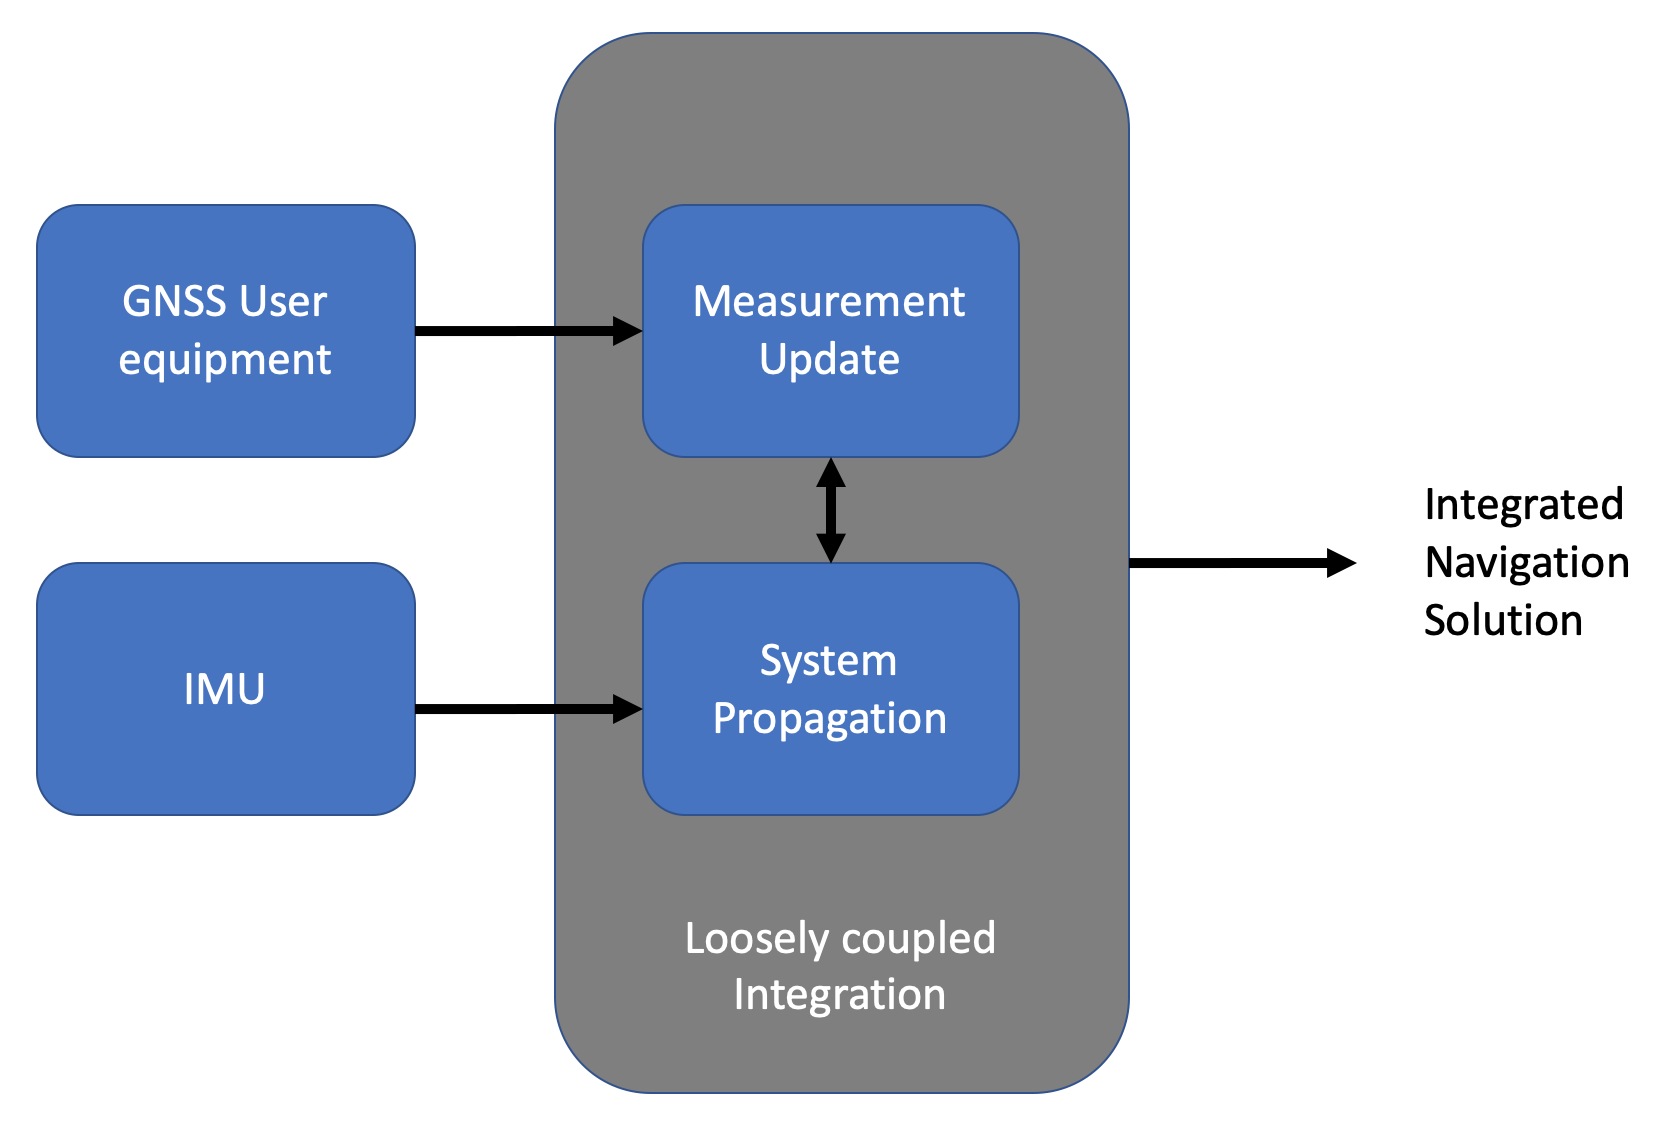
\includegraphics[width=8.5cm, height=6cm]{Images/Navigation_solution.png}
%   \caption{Navigation solution using loosely coupled integration.}
%   \label{nav_sol}
% \end{figure}

The error state propagation model is developed for the Kalman filter were attitude, position, velocity, accelerometer and gyroscope biases, are estimated with respect to the inertial frame.

\begin{equation}
x^{i}_{INS} = \left( \begin{matrix} \delta\Psi \\ \delta v  \\ \delta r \\ b_{a} \\ b_{g} \end{matrix} \right) \label{eskf_states}
\end{equation}

\noindent in \eqref{eskf_states}, $\delta\Psi$, $\delta v$, $\delta r$ are the attitude represented by Euler angles, position and velocity, whereas $b_{a}$ and $b_{g}$ the biases, all represented in $\mathbb{R}^{3}$ respectively. The nonlinear state propagation equations are described as:

\begin{align}
R^{i}_{b} &= R^{i-}_{b} (I_{3} + \Omega_{b}\tau) \\
v^{i}     &= v^{i-} + R^{i}_{b}(a_{b}-b_{a})\tau + g\tau \\
r^{i}     &= r^{i-} + v^{i}\tau + (R^{i}_{b}(a_{b}-b_{a}) + g) \frac{\tau^{2}}{2} \\
b_{a}     &= b^{-}_{a}\\
b_{g}     &= b^{-}_{g}
\end{align}

\noindent where the $x^{-}$ symbol assigned to the variables refers to the value from the previous step, $R^{i}_{b}$ is the direction cosine matrix that maps the accelerometer measurements $a_{b}$ from the body frame to the inertial frame, $b_{a}$ and $b_{g}$ are the accelerometer and gyroscope biases, $\Omega_{b}$ is the skew symmetric form of the angular velocities, $\tau$ is the time step. Finally $v^{i}$ and $r^{i}$ correspond to the velocity and the position of the vehicle in the inertial frame, respectively.

The Jacobian transition matrix $F^{i}$, the error covariance matrix $P$, the system noise covariance matrix $Q$, the measurement noise covariance matrix $R$ and observation matrix $H$ were defined as follows:

\begin{equation}
F^{i} = \left[ \begin{matrix}                         I_{3}  &     0_{3} & 0_{3} &         0_{3} & R^{i}_{b}\tau \\
                    [-(R^{i}_{b}(a_{b}-b_{a})+g)\wedge]\tau  &     I_{3} & 0_{3} & R^{i}_{b}\tau &         0_{3} \\
                                                        0_{3} & I_{3}\tau & I_{3} &         0_{3} &         0_{3} \\
                                                        0_{3} &     0_{3} & 0_{3} &         I_{3} &         0_{3} \\
                                                        0_{3} &     0_{3} & 0_{3} &         0_{3} &         I_{3} 
                \end{matrix} \right] \label{eskf_f}
\end{equation}

\begin{equation}
P = Q = \left[   \begin{matrix} \alpha^{2}_{g} &          0_{3} & 0_{3} &           0_{3} &           0_{3} \\
                                        0_{3} & \alpha^{2}_{a} & 0_{3} &           0_{3} &           0_{3} \\
                                        0_{3} &          0_{3} & 0_{3} &           0_{3} &           0_{3} \\
                                        0_{3} &          0_{3} & 0_{3} & \alpha^{2}_{ba} &           0_{3} \\
                                        0_{3} &          0_{3} & 0_{3} &           0_{3} & \alpha^{2}_{bg} 
                \end{matrix} \right] \label{eskf_pq}
\end{equation}

\begin{equation}
R = \left[    \begin{matrix} \alpha^{2}_{x} &          0_{3} &          0_{3} \\
                                        0_{3} & \alpha^{2}_{y} &          0_{3} \\
                                        0_{3} &          0_{3} & \alpha^{2}_{z}  
                \end{matrix} \right] \label{eskf_r}
\end{equation}

\begin{equation}
H = \left[    \begin{matrix} 0_{3} & 0_{3} & I_{3} & 0_{3} & 0_{3} \end{matrix} \right] \label{eskf_h}
\end{equation}

\noindent In \eqref{eskf_f}, $[x]\wedge$ represents the skew symetric matrix form of the vector $x$, $I_{3}$ and $0_{3}$ are the $3\times 3$ identity and zero matrices. In \eqref{eskf_pq} $\alpha^{2}_{g}$, $\alpha^{2}_{a}$, $\alpha^{2}_{ba}$ and $\alpha^{2}_{bg}$, are the power spectral densities or error standard deviation of the gyro random noise, accelerometer random noise, accelerometer bias variation and gyroscope bias variation. The values of $\alpha^{2}_{x}$, $\alpha^{2}_{y}$ and $\alpha^{2}_{z}$ in \eqref{eskf_r} are the noise standard deviation for each axis of the sensor input. Finally the matrix \eqref{eskf_h} is the measurement matrix which maps form the sensor measurements to the states. In practice, the values of the standard deviations were obtained from the manufacturer sensor datasheets.

\subsection{IBVS}
As stated in \cite{corke}, the task of visual servoing is to control the pose of a robot relative to the goal, using its visual features that have been extracted from an image. Image based visual-servoing (IBVS) uses this features directly and the control is performed in image coordinate space $\mathbb{R}^{2}$. The challenging control problem using IBVS is that the image features have a highly nonlinear relation to the camera pose.

\begin{figure}
\centering
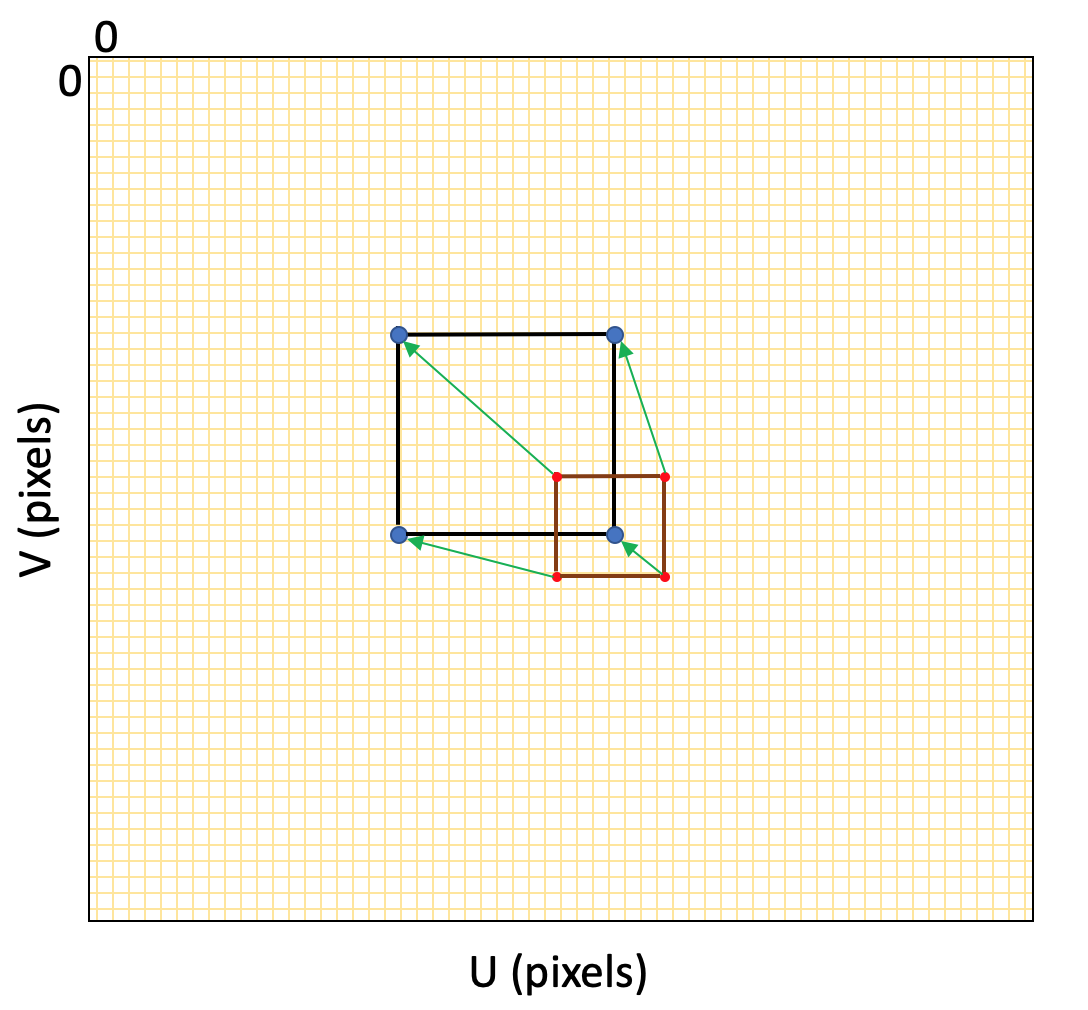
\includegraphics[width=6.5cm, height=6cm]{Images/ibvs_goal.png}
\caption{IBVS example, where black square with blue dots is the desired view and the red square whit red dots are the current view.}
\label{ibvs_goal}
\end{figure}

Using Fig. \ref{ibvs_goal} as example, the goal is to move the measured feature points and make them coincide with the desired points. The camera mounted system will need to perform a pose control in order to make that the target feature points achieve the goal.

\begin{align}
p & = \textit{p}(P,K,R_{c}) \label{img_proj} \\
\dot{p} & = J_{p}(P,K,R_{c})v \label{img_proj_jac}
\end{align}

Considering the perspective projection equation in \eqref{img_proj} and its derivative in \eqref{img_proj_jac} (also known as $\textit{image Jacobian}$), we can see that the camera motion results in different motion on the image points. In this way moving a camera with a body velocity in the world frame $v=(\textit{v}, \omega)$ and observing a point $P$ with camera relative coordinates $P=(X,Y,Z)$, an estimate of a point velocity can be obtained by $\dot{P} = -\omega \times P - v$. Taking into account the normalized image-plane coordinates, its time derivative and mapping them to pixel coordinates, we get:

\begin{equation}
\begin{bmatrix} \dot{\bar{u}} \\ \dot{\bar{v}} \end{bmatrix}  = \begin{bmatrix} -\frac{f}{\rho_{u}Z} & 0 & \frac{\bar{u}}{Z} & \frac{\rho_{v}\bar{v}}{\rho_{u}} \\ 0 & -\frac{f}{\rho_{v}Z} & \frac{\bar{v}}{Z} & -\frac{\rho_{u}\bar{u}}{\rho_{v}} \end{bmatrix} \begin{bmatrix}  V_{x} \\ V_{y} \\ V_{z} \\ \omega_{z} \end{bmatrix} \label{pixel_vels}
\end{equation} 

In \eqref{pixel_vels}, $\bar{u},\bar{v}$ are the pixel coordinates relative to the principal point ($u_{0},v_{0}$). $\rho_{u}, \rho_{v}$ are the pixel dimensions and $f$ is the focal length. The matrix $J_{p}(p,Z)$ is a $2 \times 6$ image Jacobian matrix for a point feature at coordinate $p$ and at distance $Z$. The angular velocities for $\omega_{x}$ and $\omega_{y}$ are removed from \eqref{pixel_vels} due to the fact that the quadrotor is an under actuated system.
Using four points as in Fig. \ref{ibvs_goal} will lead to:

\begin{equation}
\left[ \begin{matrix}
    \dot{u_{1}} \\ \dot{v_{1}} \\ \dot{u_{2}} \\ \dot{v_{2}} \\ \dot{u_{3}} \\ \dot{v_{3}} \\ \dot{u_{4}} \\ \dot{v_{4}} \end{matrix}  \right] = \left[ \begin{matrix} J_{p}(p_{1},Z_{1}) \\ J_{p}(p_{2},Z_{2}) \\ J_{p}(p_{3},Z_{3}) \\ J_{p}(p_{4},Z_{4}) \\ \end{matrix} \right] v \label{point_motion}
\end{equation}

Solving \eqref{point_motion} in order to get the camera velocities yields:

\begin{equation}
v = \left[ \begin{matrix} J_{p}(p_{1},Z_{1}) \\ J_{p}(p_{2},Z_{2}) \\ J_{p}(p_{3},Z_{3}) \\ J_{p}(p_{4},Z_{4}) \\ \end{matrix} \right]^{-1} \left[ \begin{matrix}
\dot{u_{1}} \\ \dot{v_{1}} \\ \dot{u_{2}} \\ \dot{v_{2}} \\ \dot{u_{3}} \\ \dot{v_{3}} \\ \dot{u_{4}} \\ \dot{v_{4}} \end{matrix}  \right] \label{camera_motion}
\end{equation}

Using the simpler linear controller $\dot{p} = \lambda(p^{\star} - p)$ we can determine the velocity, where $\lambda$ is a proportional gain and $p^{\star} - p$ are the errors between the desired points and the current points on the image, leading to the final control equation \eqref{ctrl_camera_motion}.

\begin{equation}
v = \lambda \left[ \begin{matrix} J_{p}(p_{1},Z_{1}) \\ J_{p}(p_{2},Z_{2}) \\ J_{p}(p_{3},Z_{3}) \\ J_{p}(p_{4},Z_{4}) \\ \end{matrix} \right]^{-1} (p^{\star} - p) \label{ctrl_camera_motion}
\end{equation}

\subsection{Initial depth estimation}
In order to use \eqref{ctrl_camera_motion}, the depth of each point is needed besides the desired and current points on the image. The way we estimate this depth is based on the method in \cite{DenaRuiz2017_2}, where target position estimation is performed in real-time. The implemented algorithm uses the center pixel position of a target on a image, this pixel is mapped into azimuth and elevation angles, and uses these measurements to estimate the target position with respect an inertial frame using an unscented Kalman filter. Using this estimation and knowing the current position of the quadrotor, we can obtain the relative distance between the aircraft and the target, and therefore, its magnitude.

The target estimation algorithm from \cite{DenaRuiz2017_2} requires to perform an initial trajectory, which will help to improve the estimation. In this case an ellipsoid trajectory was chosen, due to the fact that with this trajectory, the azimuth and elevation angles vary enough to give a wider range of values in both axes as shown in Fig \ref{ellipsoid_traj}.

\begin{figure}
\centering
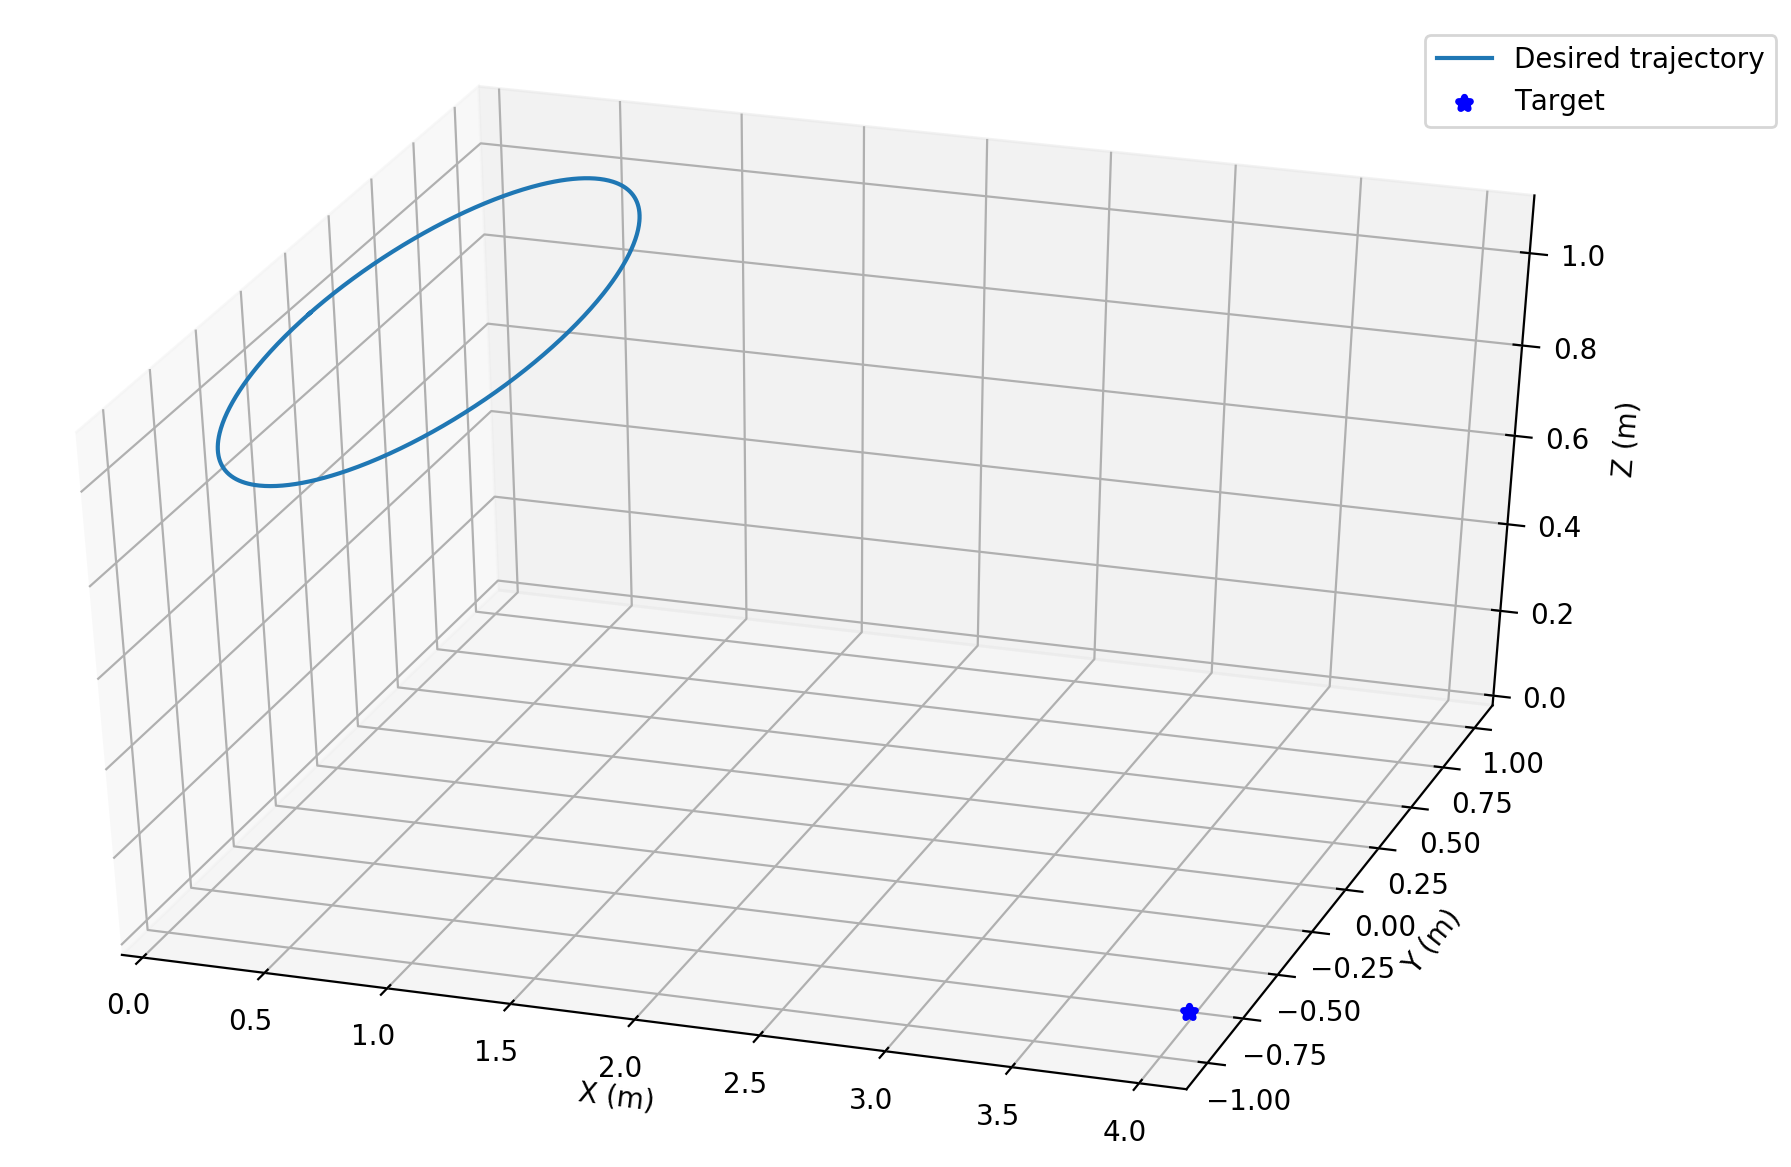
\includegraphics[width=8.0cm, height=7cm]{Images/3D_est_trajectory.png}
\caption{ellipsoid trajectory for target position estimation.}
\label{ellipsoid_traj}
\end{figure}

The dimensions of this ellipsoid trajectory are 1 m in long radius along lateral, and 0.5 m in short radius along forwards direction, and the trajectory is performed at a fixed altitude of 1m.

The selected camera onboard is the Tau2 from FLIR\textregistered, Fig.\ref{tau2} and its characteristics are described in Table \ref{tau2_params}. The images are received through the usb port of the single board computer and processed with OpenCV libraries. 

\begin{table}
\small\sf\centering
\caption{Tau2 camera intrinsic parameters and dimensions}
\scalebox{0.8}{
\begin{tabular}{c c}
\toprule
    Spec & value\\
\midrule
    Frame rate(fps) & 30 \\
    Resolution(pixels) & 640$\times$512\\
    Spectral Band($\mu$ m) & 7.5-13.5\\
    Pixel size($\mu$ m) & 17\\
    Focal Length(mm) & 7 \\
    Physical dimensions(mm) & $40\times40\times15$\\
\bottomrule
\end{tabular}}
\label{tau2_params}
\end{table}

\section{Experimental validation}
\subsection{Setup}
The entire setup to validate the proposed architecture is based on \cite{DenaRuiz2017_1} and \cite{DenaRuiz2017_2}, where a Pelican quadrotor from AScTec as shown in Fig. \ref{pelican} is used as the aerial vehicle. Experiments are performed in indoor conditions and Motive Optitrack is used to retrieve the drone position. These measurements are configured to emulate the GPS measurements. Communication between the drone and the Optitrack system is established through a local network and the Robot Operating System (ROS). As a representative to landmark, a heating pad as shown in Fig.\ref{tgt} is used, which is heated up to 30°C and lying completely on the floor.

\begin{figure}%[!t]
\begin{tabular}[b]{cc}
    \begin{tabular}[b]{c}
    \begin{subfigure}[b]{0.45\columnwidth}
        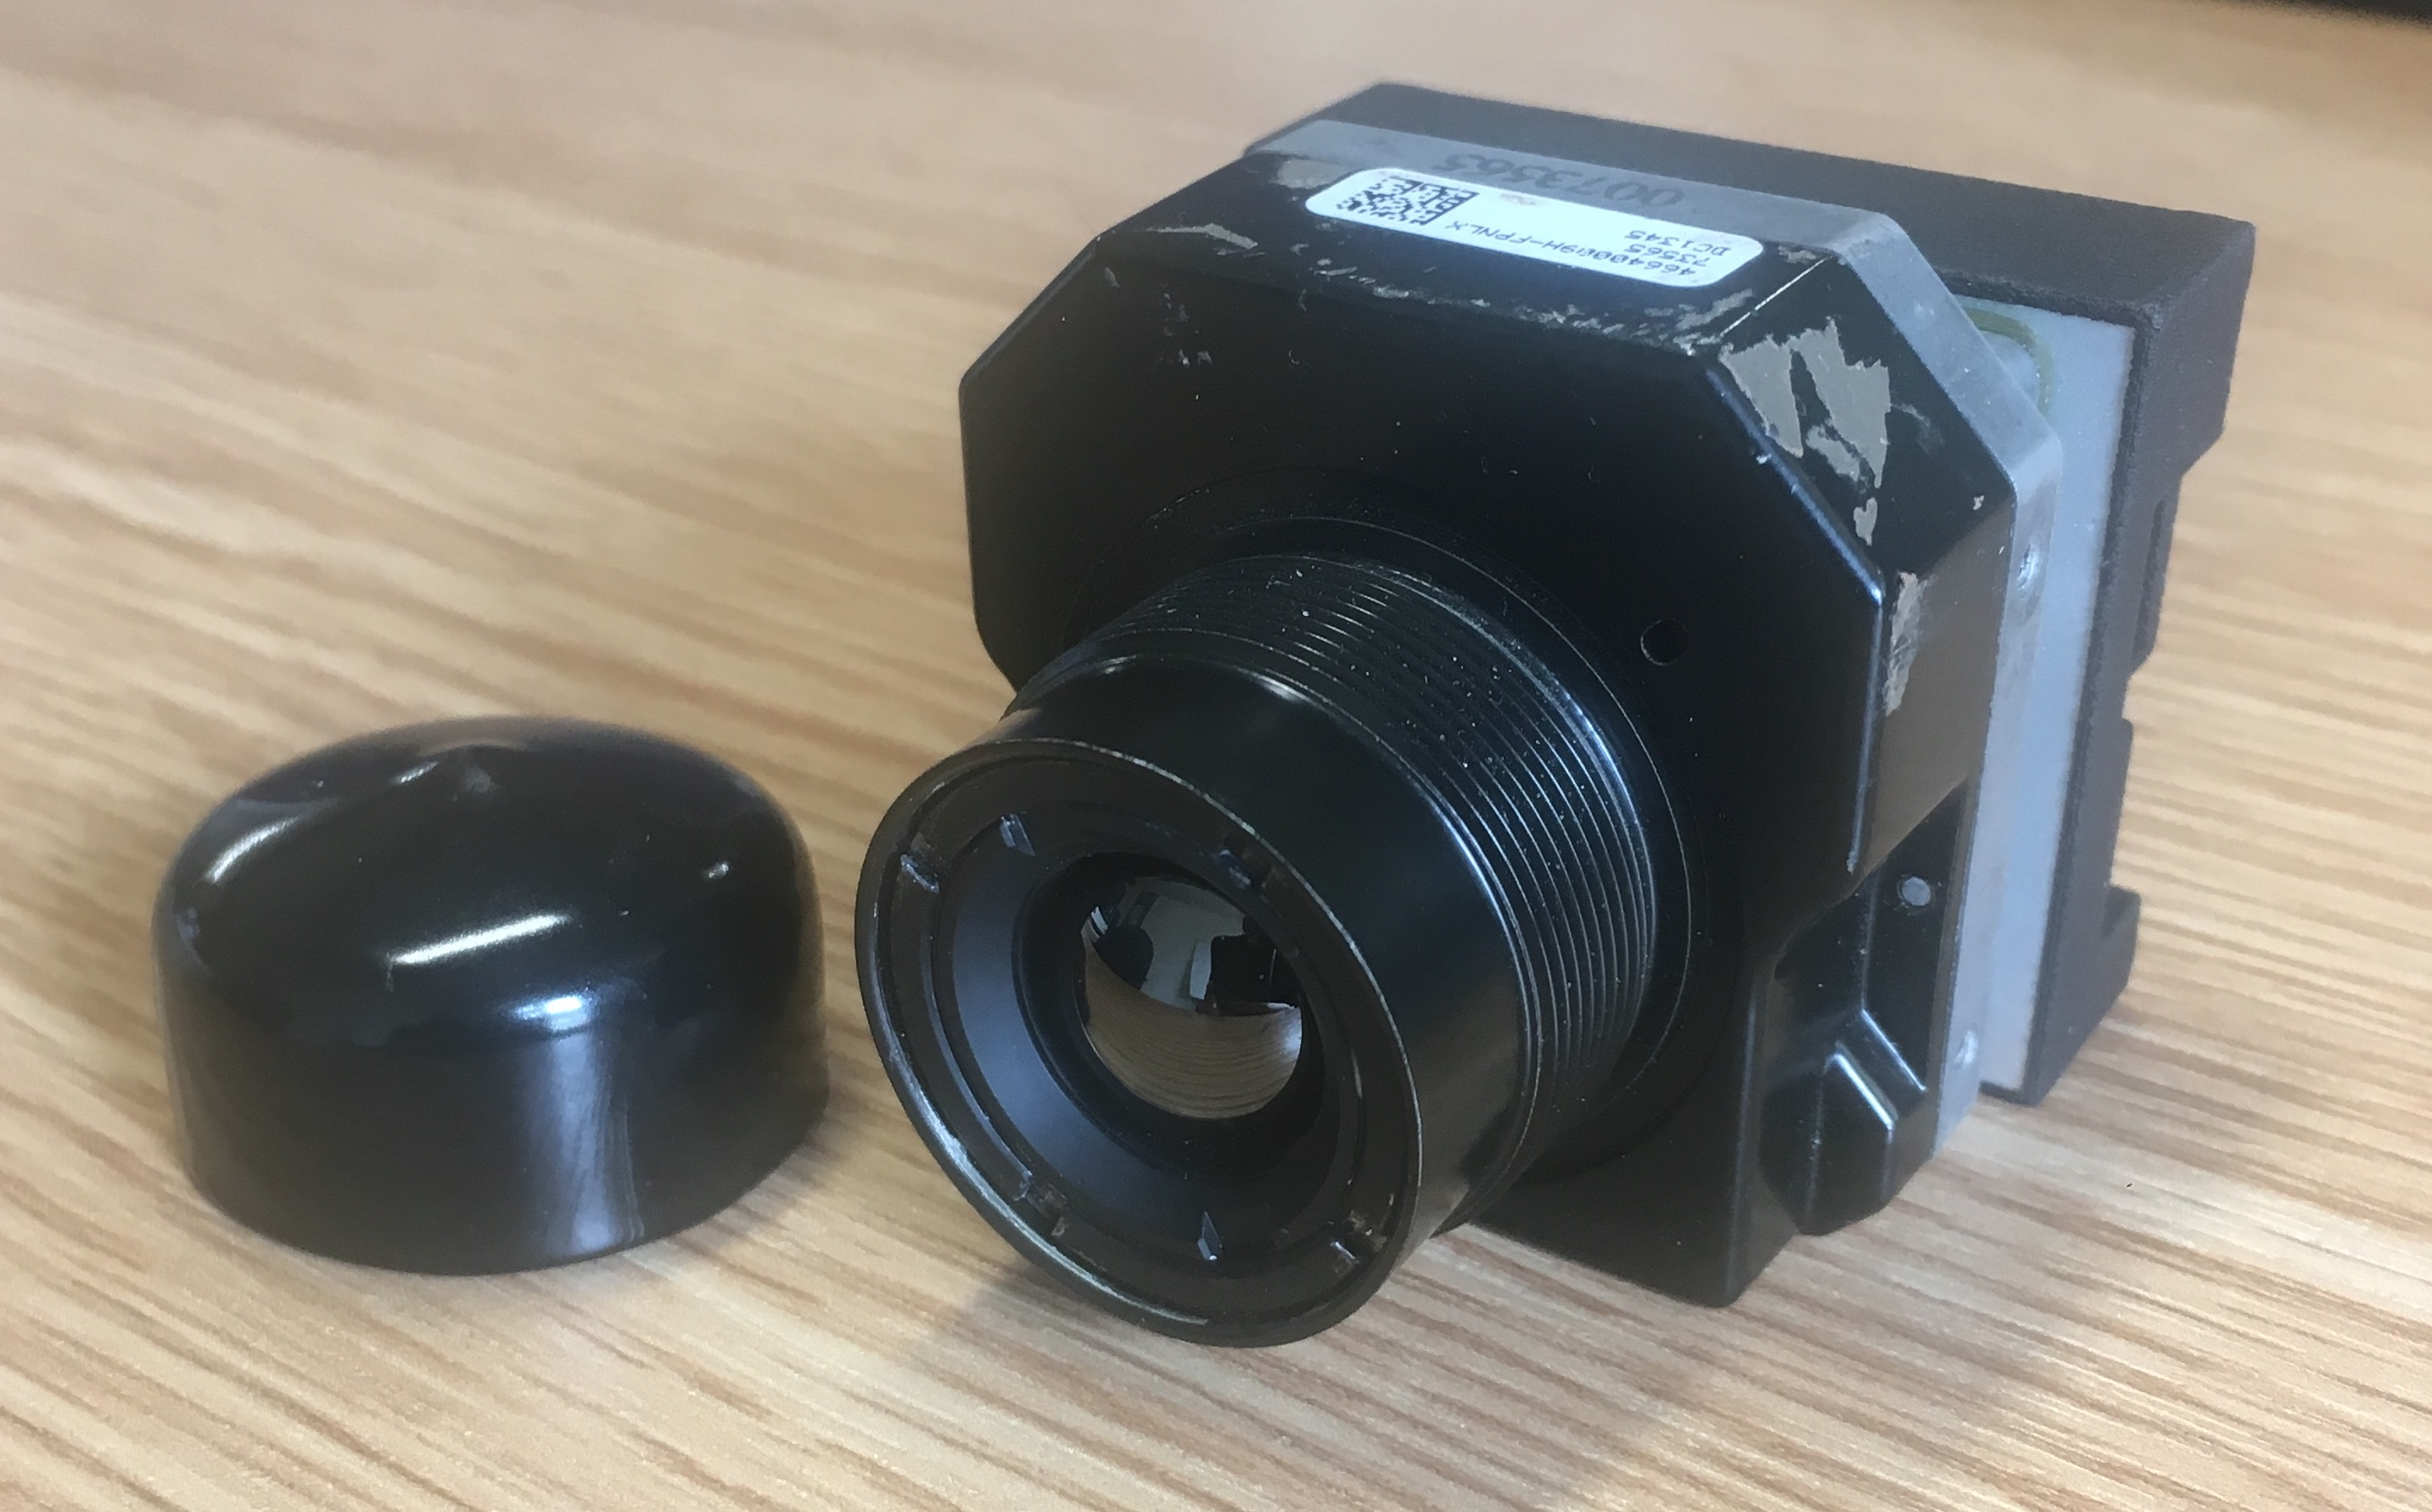
\includegraphics[width=\textwidth]{Images/flir_tau2.jpg}
        \caption{Thermal camera FLIR Tau2.}
        \label{tau2}
    \end{subfigure}\\
    \begin{subfigure}[b]{0.45\columnwidth}
        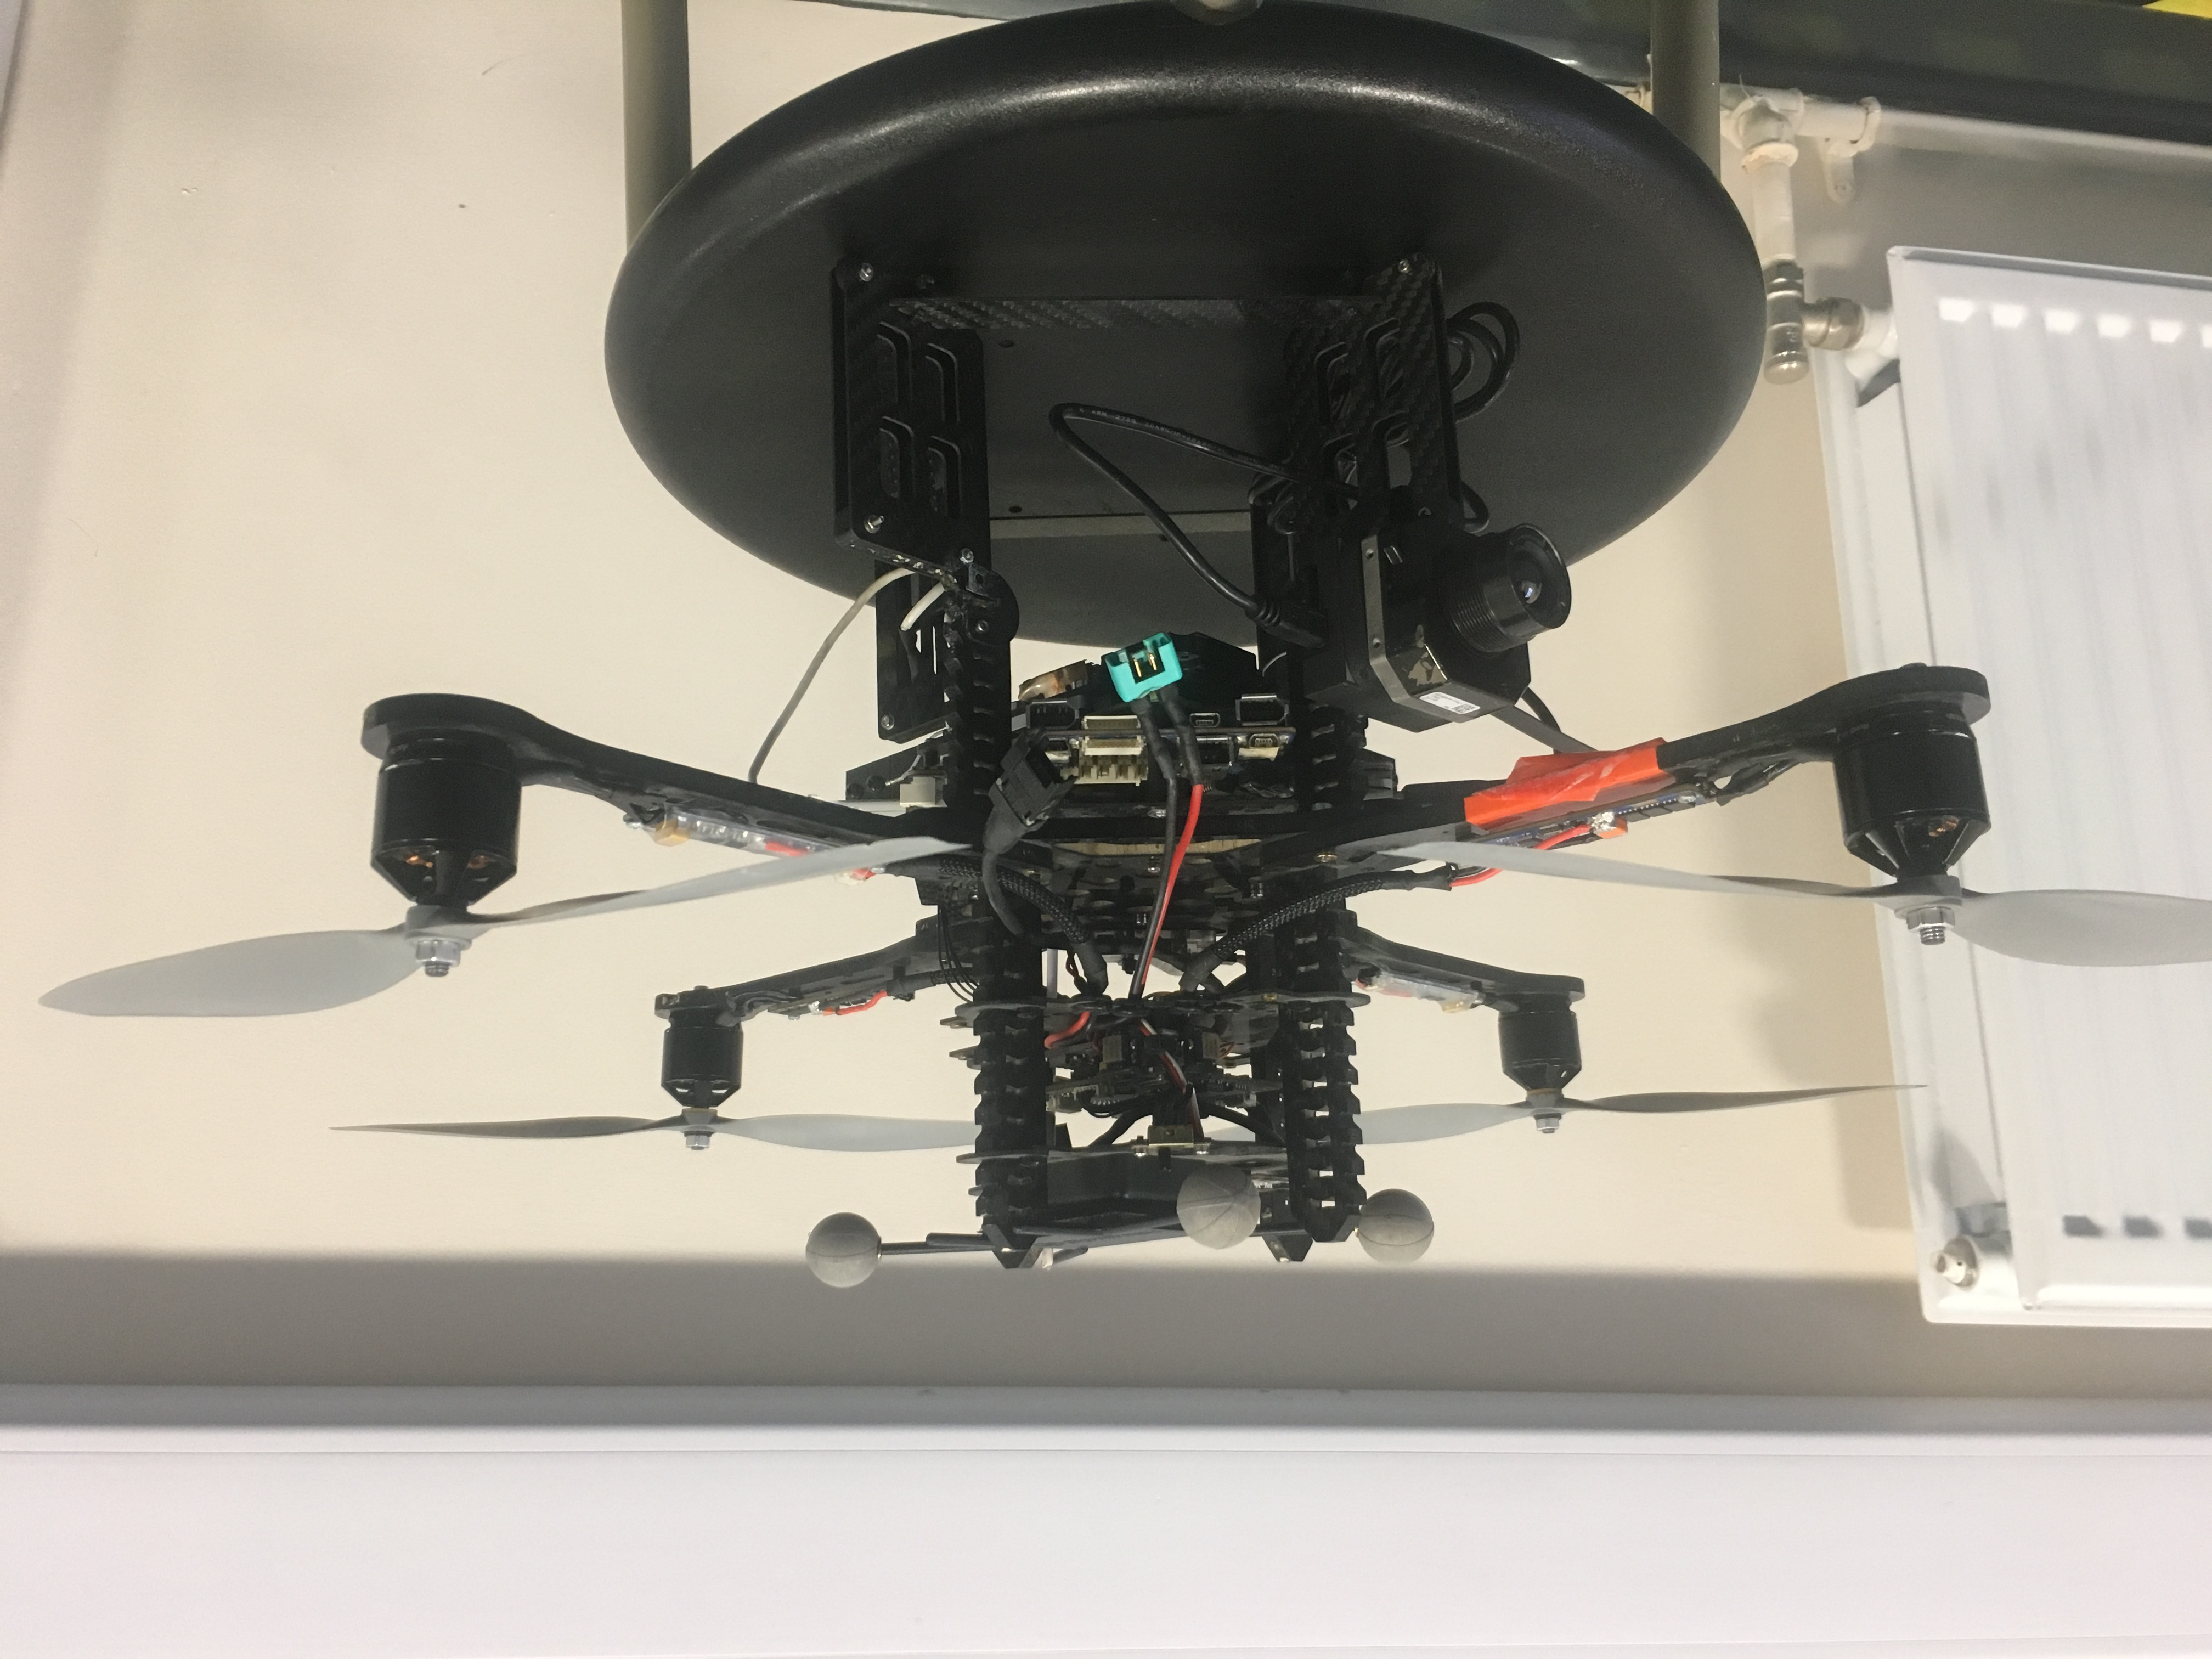
\includegraphics[width=\textwidth, angle=180]{Images/pelican.jpg}
        \caption{AscTEc Pelican quadrotor.}
        \label{pelican}
    \end{subfigure}
    \end{tabular}
    &
    \begin{subfigure}[b]{0.5\columnwidth}
    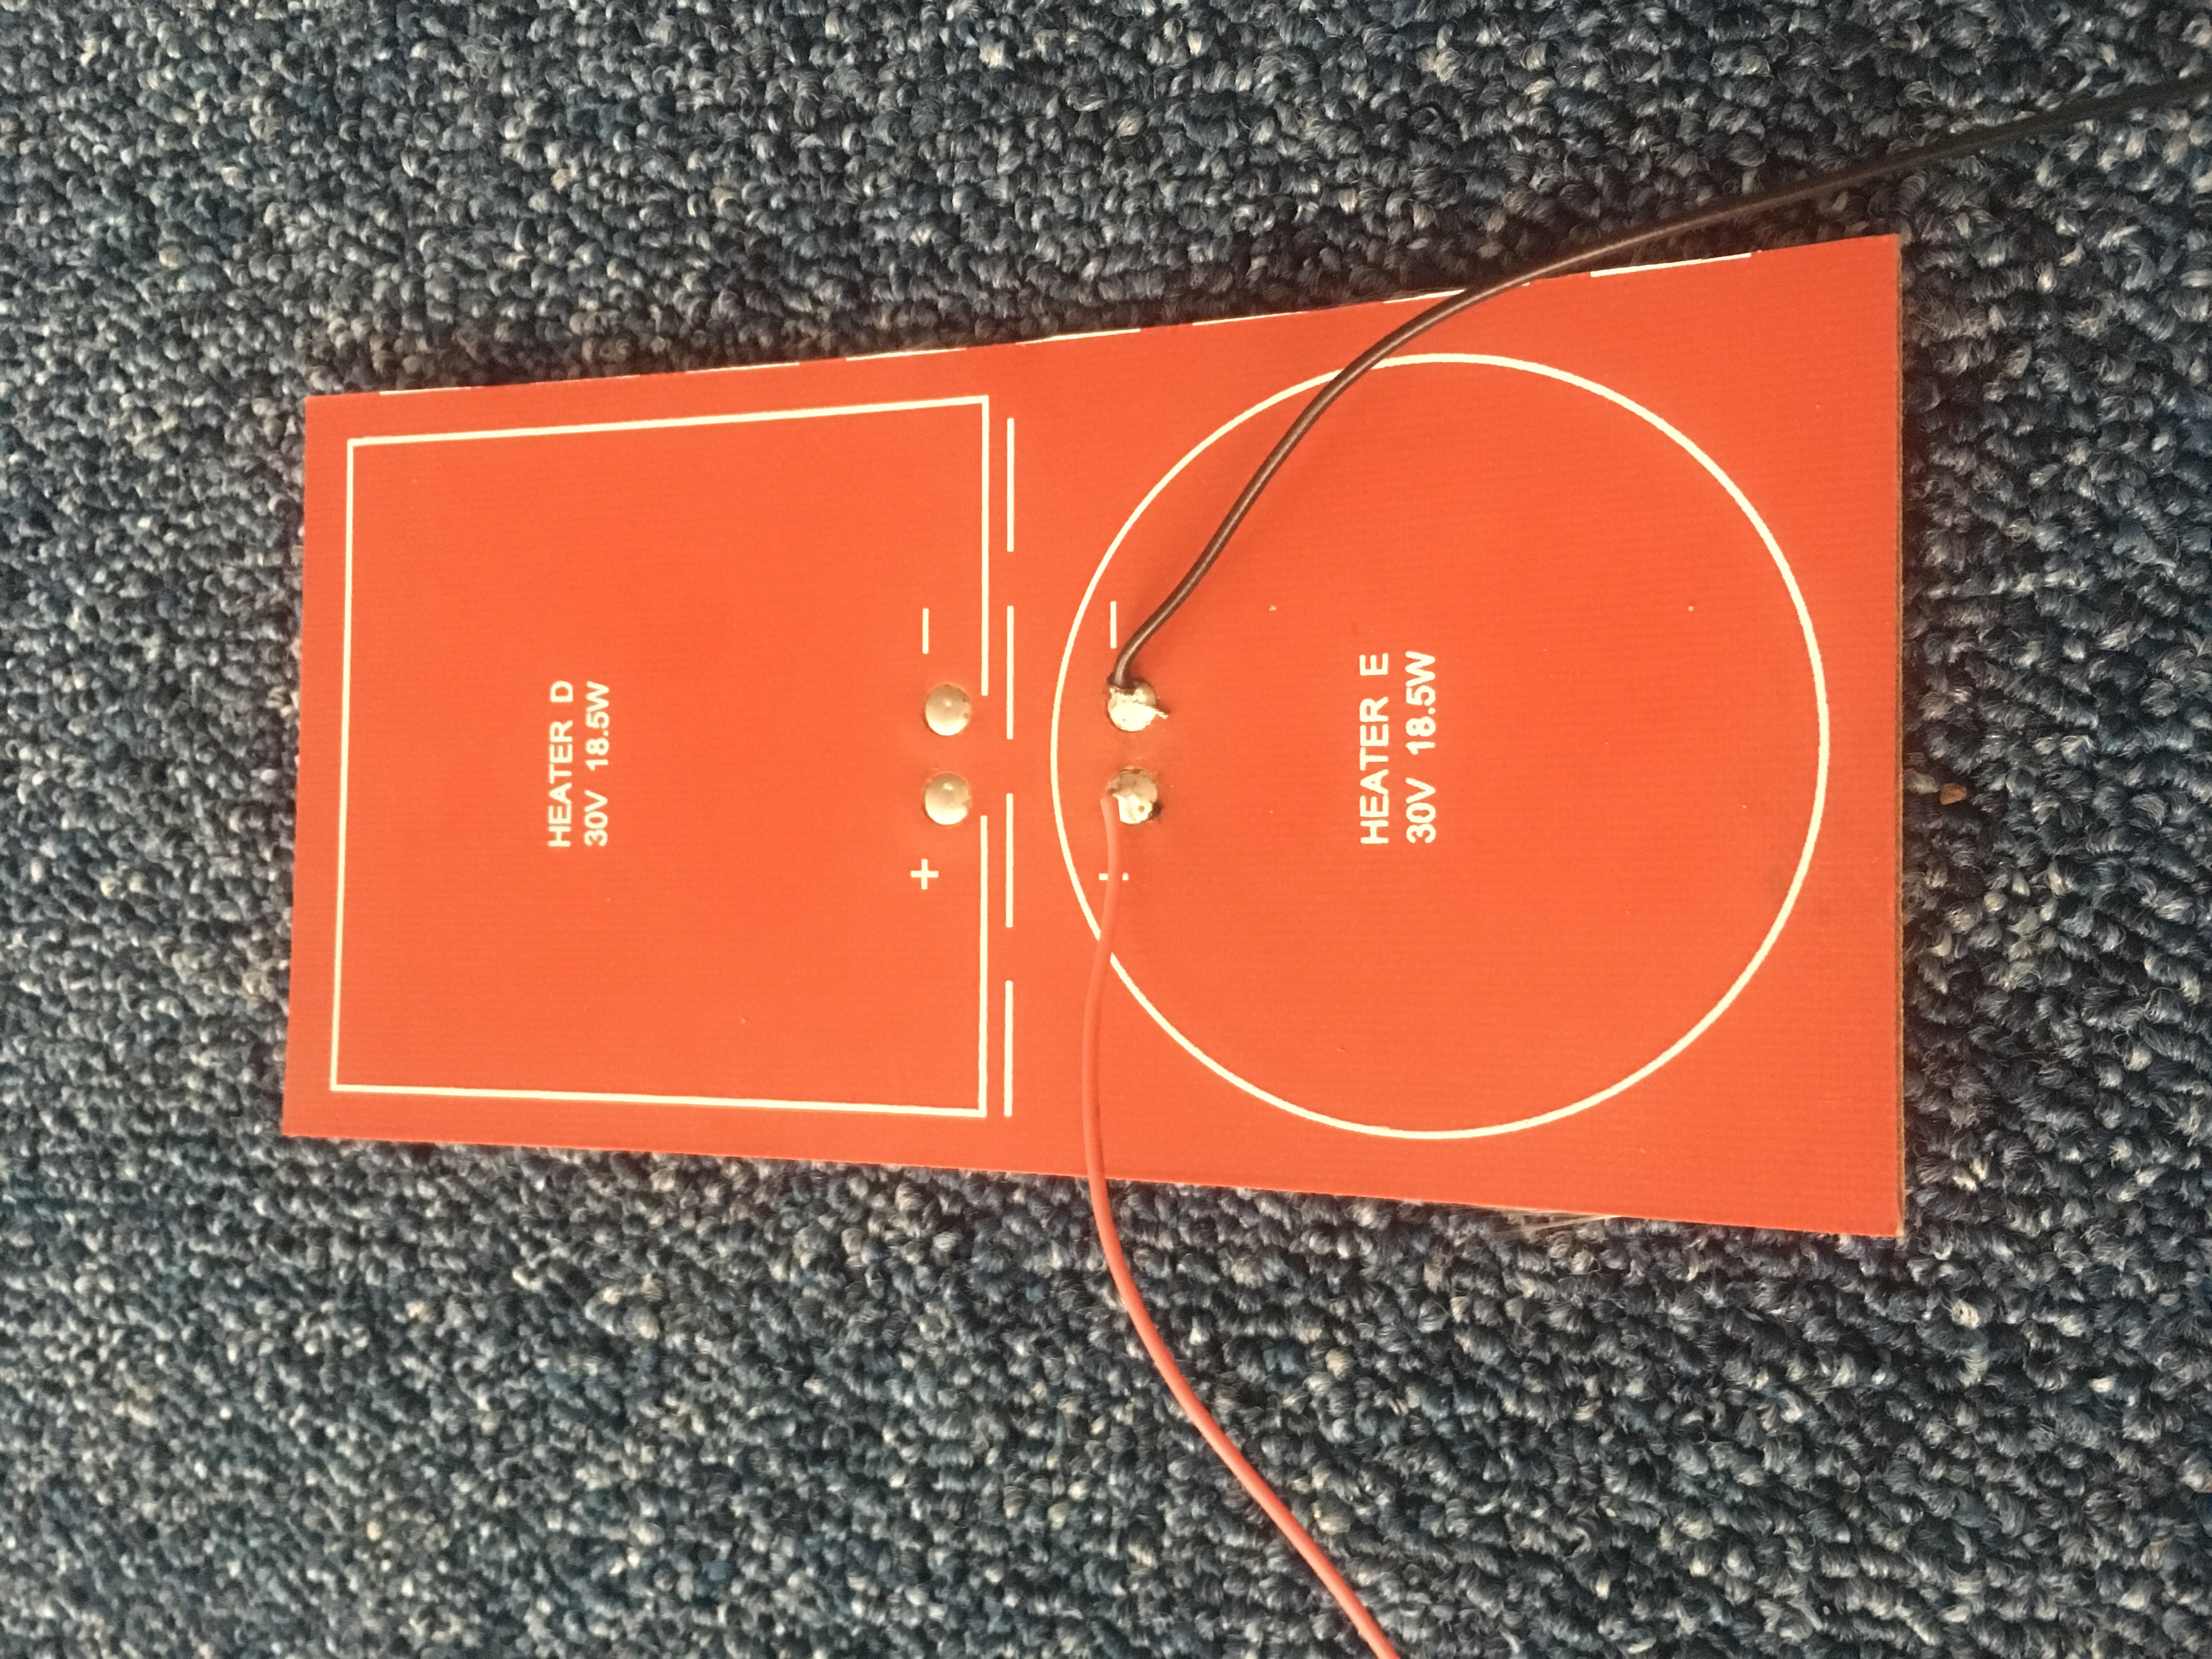
\includegraphics[width=\textwidth, angle=270]{Images/thermal_tgt.jpg}
    \caption{Thermal PAD used as \\
             the thermal target for \\
             IBVS.}
    \label{tgt}
    \end{subfigure}
\end{tabular}
\label{fig:ABC}
\caption{Main elements of the setup scenario.}
\end{figure}


Images coming from the thermal camera are received and mapped into HSV format, where the pixel intensity from the heated target are recorded and extracted from the non-desired objects using inRagne algorithm. In order to remove any other similar pixel intensities, the image is filtered by the erode and dilate algorithms. For the IBVS, the image used for target position estimation is utilized. Using the contours and bounding rect algorithm, the maximum and minimum four pixel points are extracted. These points are depicted in black, whereas the desired points are in yellow, in Fig. \ref{img_proj}.

\begin{figure}
\centering
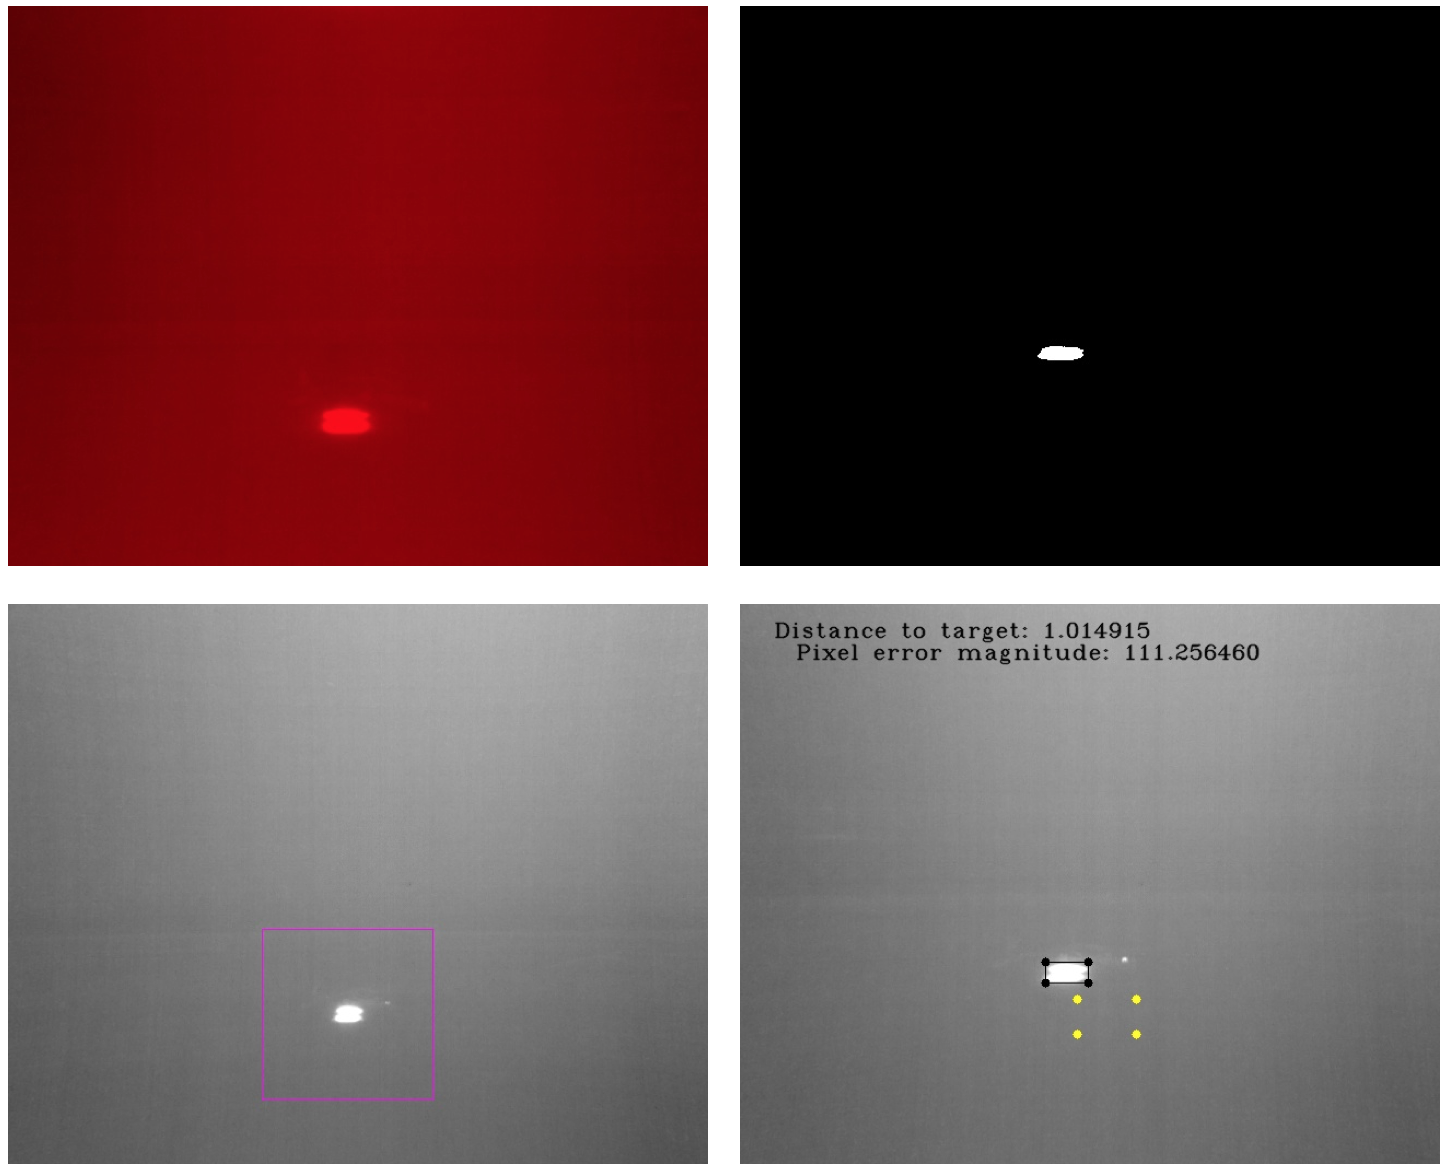
\includegraphics[width=8.5cm, height=7cm]{Images/image_proc.jpg}
\caption{Different image processing for target tracking and IBVS. Image in HSV in top left, on top right the output of inRange in black and white. On bottom left the object tracking and region of interest in red for tracking, finally on bottom right the desired point in yellow and the target pixels.}
\label{img_proc}
\end{figure}

\subsection{Results}
The full experiment is composed of two stages: initial depth estimation and image based visual servoing. The first stage consists in performing the target estimation using the visual measurements form the thermal images of the target. The central pixel from the target is found, this pixel position is mapped into the bearing angles (azimuth and elevation), treating these angles as the measurements, the target position estimation is performed. The thermal target was placed on the floor, in the position ($X=4.0$, $Y=-0.8$, $Z=0.0$) with respect to the inertial frame selected as the initial position of the quadrotor. To perform the depth estimation, the initial values are designated as $\hat{X} = \left[10, 10, 10\right]$, $Q = 0_{3}$ and the following matrices for process model, error covariance and measurement noise covariances are selected.

\begin{equation*}
P = \begin{bmatrix} 20 & 0 &  0\\
                    0 &20 &  0\\
                    0 & 0 & 20 \end{bmatrix},
F = \begin{bmatrix}  1 & 0 &  0\\
                    0 & 1 &  0\\
                    0 & 0 &  1 \end{bmatrix}
\end{equation*}

\begin{equation*}
R = \begin{bmatrix}  0.1^{2} & 0 \\
0 & 0.06^{2} \end{bmatrix}
\end{equation*}

For the IBVS, the controller gain is chosen as $\lambda = 0.05$, based on an empirical tuning. For the navigation solution using the error state Kalman filter, the covariance matrices values are $\alpha_{g} = diag([0.008^{2} 0.009^{2} 0.008^{2}])$, $\alpha_{a} = diag([0.05^{2} 0.03^{2} 0.02^{2}])$, $\alpha_{bg} = diag([(8.7\times10^{-5})^{2} (8.7\times10^{-5})^{2} (8.7\times10^{-5})^{2}])$, $\alpha_{ba} = diag([(39\times10^{-5})^{2} (39\times10^{-5})^{2} (39\times10^{-5})^{2}])$ and $\alpha_{ba} = diag([0.25^{2} 0.25^{2} 0.25^{2}])$. These values are calculated from experimental data, recording the accelerometer and gyroscope measurements when the IMU is resting on a flat surface.

\begin{figure}
\centering
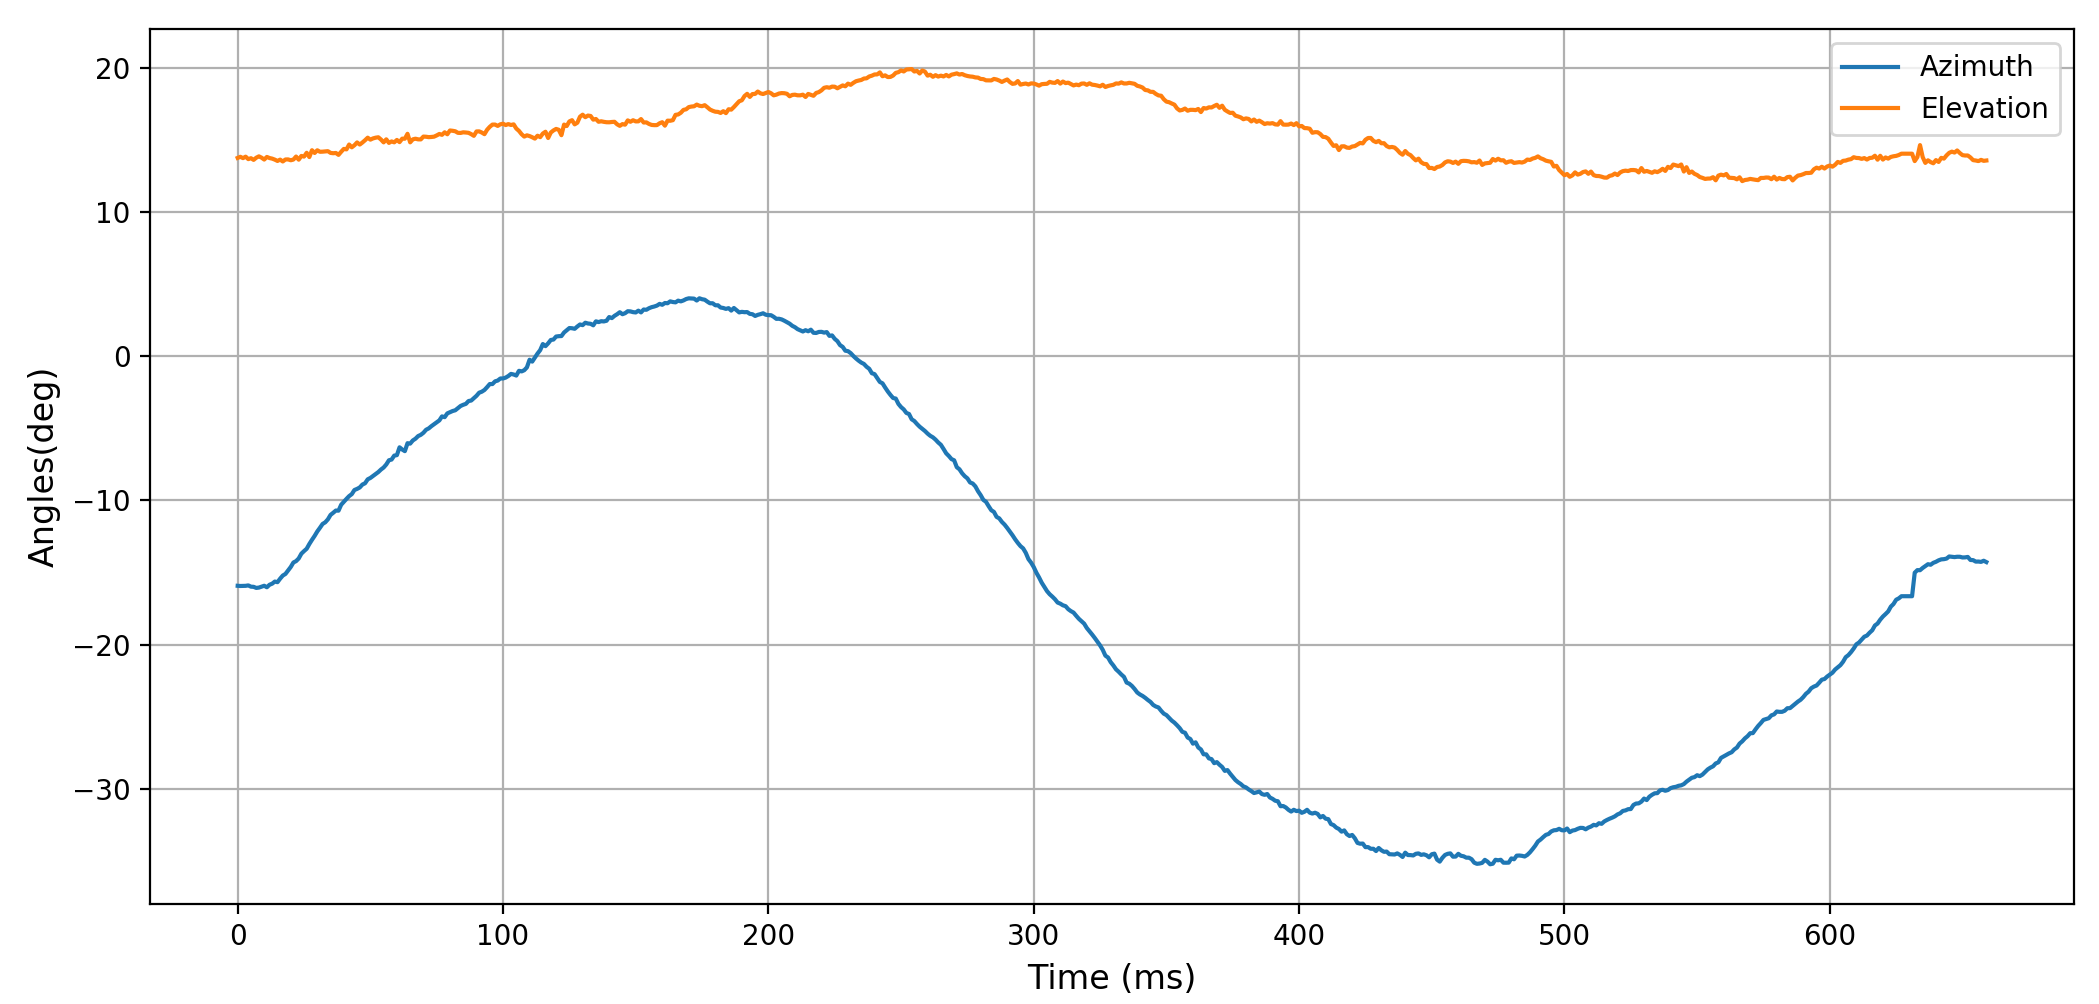
\includegraphics[width=8.5cm, height=4.5cm]{Images/azimuth_elevation.png}
\caption{Azimuth and elevation angles obtained from the pixel tracking position.}
\label{azimuth_elevation}
\end{figure}

\begin{figure}
\centering
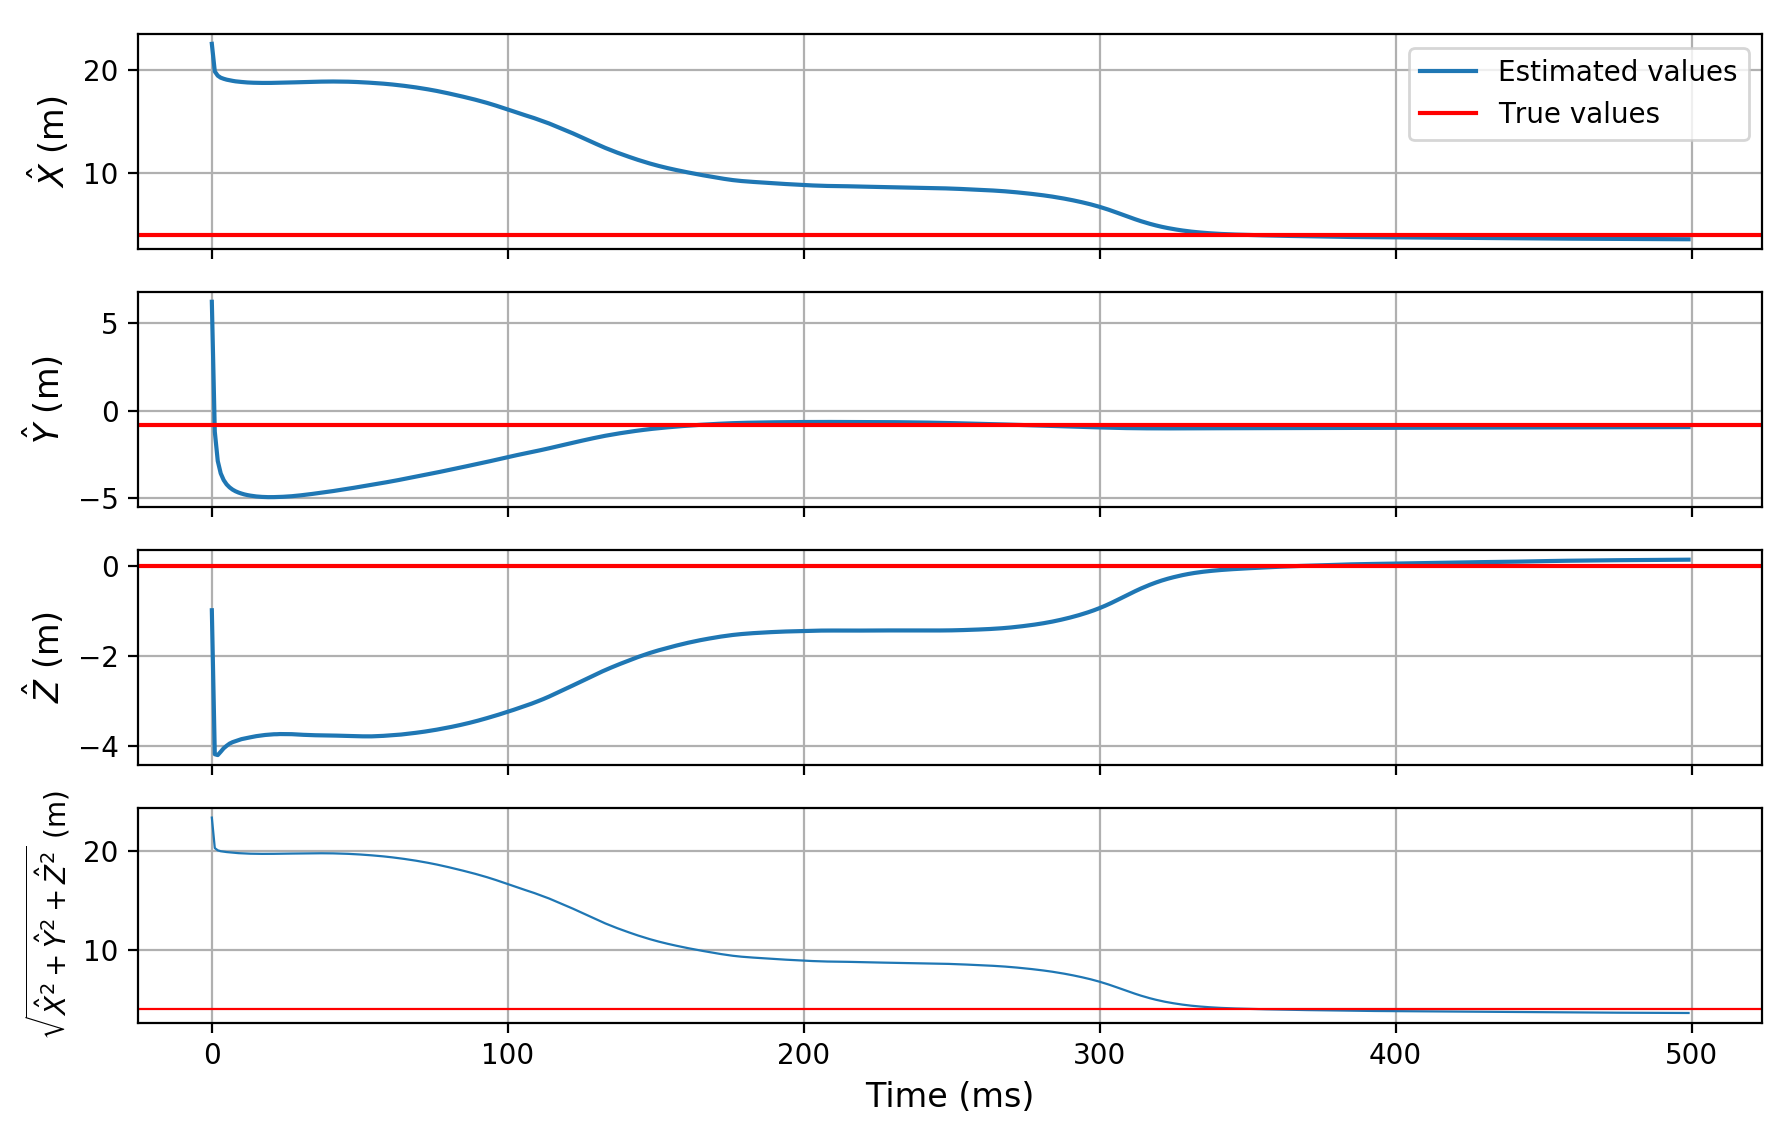
\includegraphics[width=8.5cm, height=7cm]{Images/tgt_depth_est.png}
\caption{Position and depth estimation in stage one.}
\label{tgt_depth_est}
\end{figure}

Once the depth has been estimated, this value is used as an initial depth estimate to perform the IBVS in stage 2. The drone changes from position to velocity control, following the desired velocity commands generated by the IBVS algorithm. The velocity results and the pixel errors are depicted on Figs. \ref{ibvs_vels}-\ref{final}. It is observed that although the drone gets closer to the ground as it approaches to the target, the errors in altitude is limited due to successful control actions including ground effect compensation. The total drone trajectory including stage 1 and 2, is shown in Fig. \ref{full_drone_traj}. 

\begin{figure}
\centering
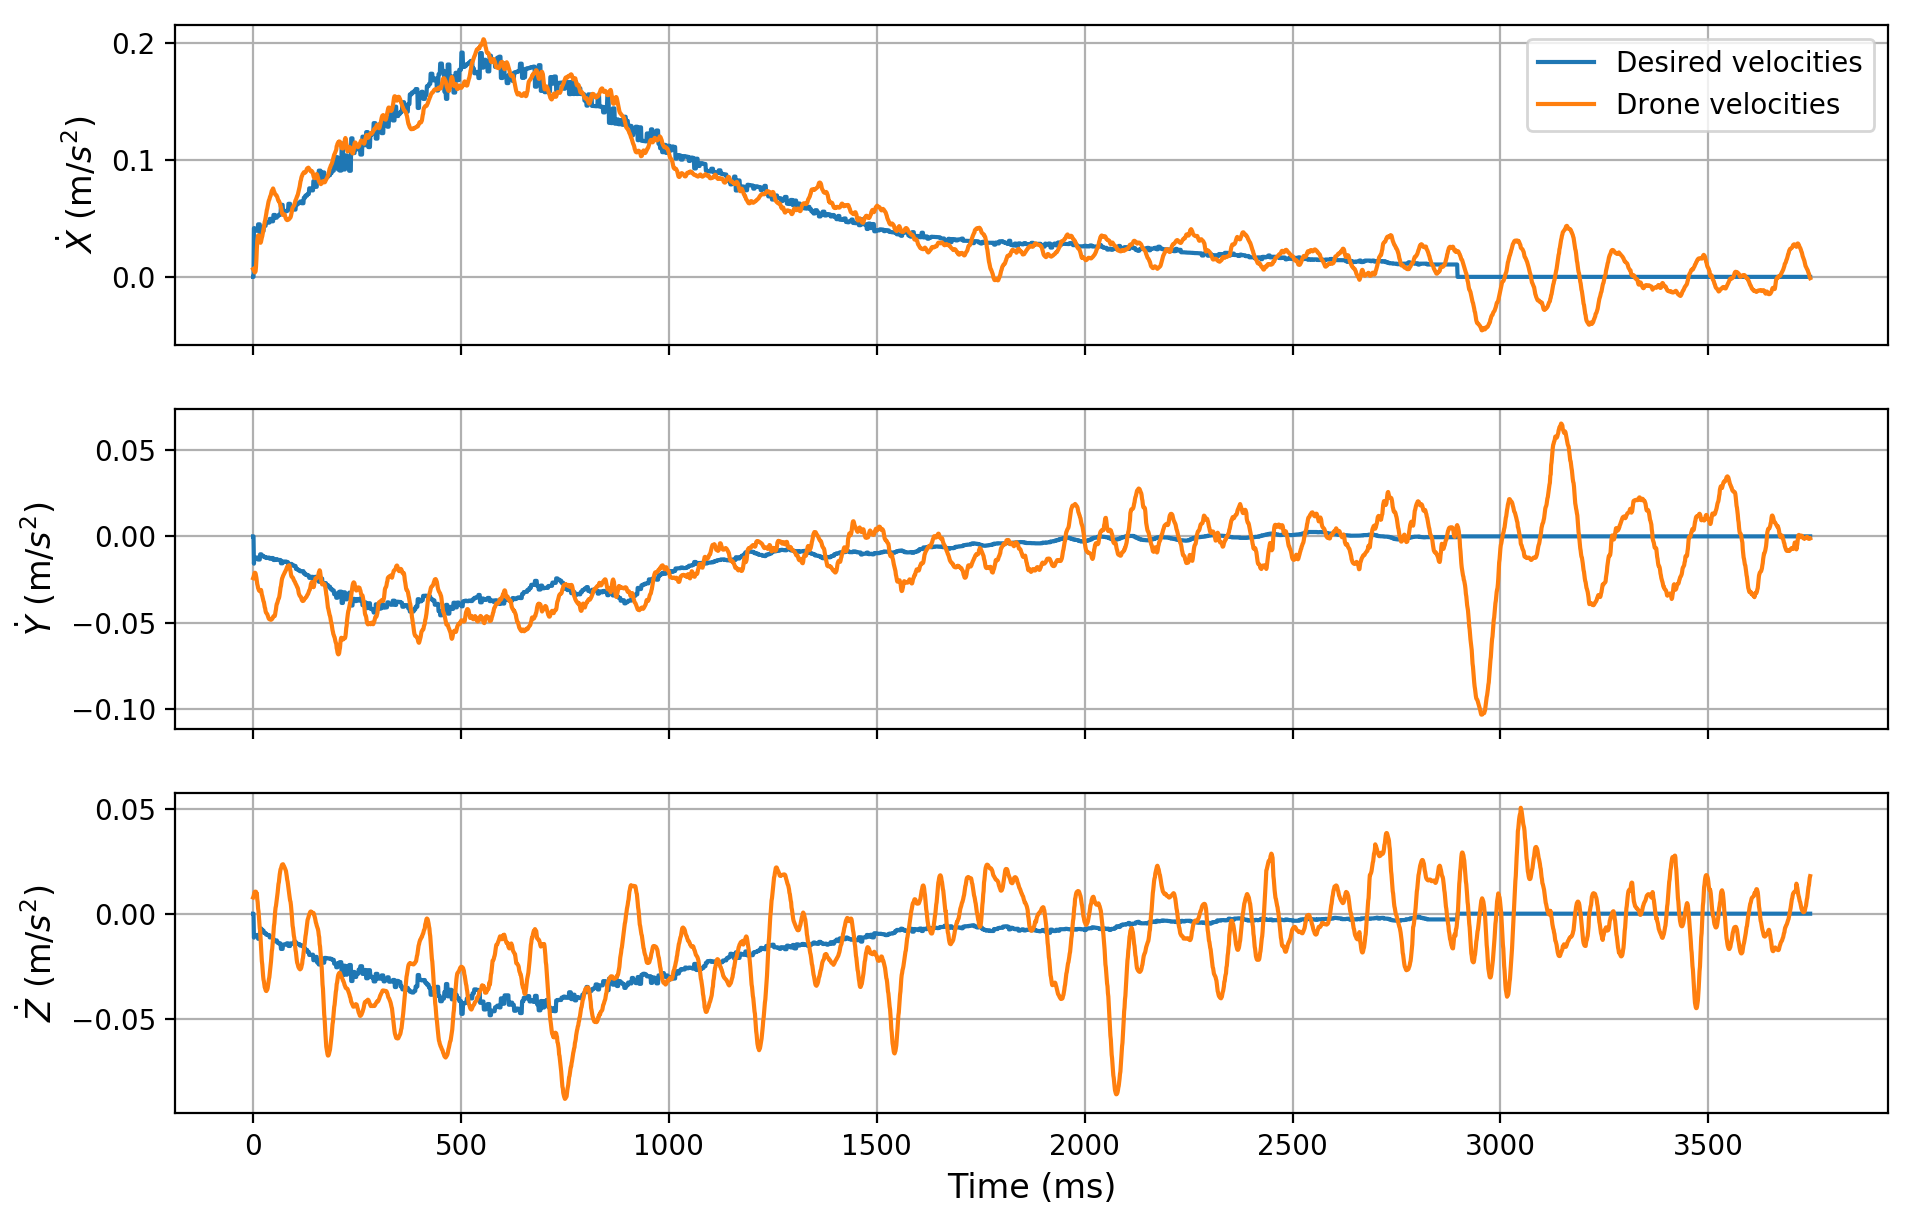
\includegraphics[width=8.5cm, height=7.5cm]{Images/velocities_stage2.png}
\caption{IBVS desired velocities vs drone velocities during stage 2 of the experiment.}
\label{ibvs_vels}
\end{figure}

\begin{figure}
\centering
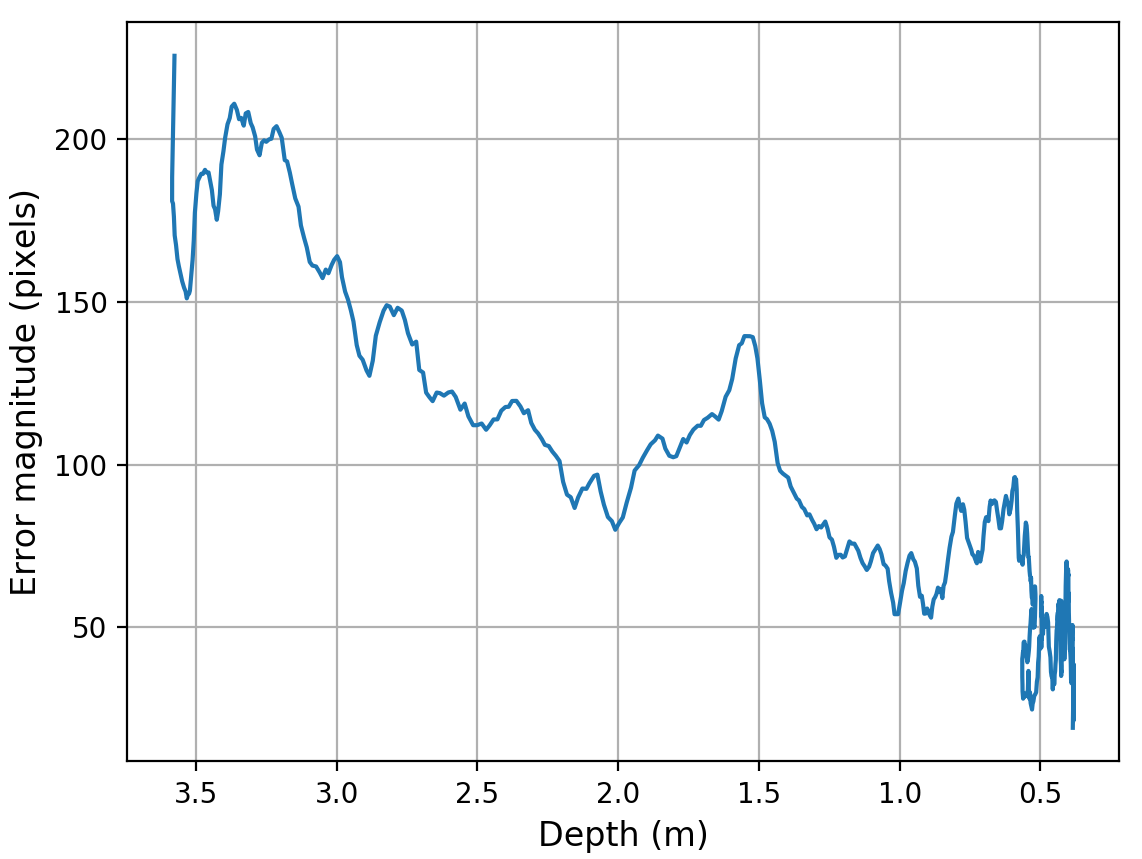
\includegraphics[width=8cm, height=7cm]{Images/pixel_error_mag.png}
\caption{Overall pixel error $\sqrt{px_{1}^{2}+px_{2}^{2}+px_{3}^{2}+px_{4}^{2}}$, during the IBVS velocity trajectory.}
\label{pixel_error}
\end{figure}

% \begin{figure}
% \centering
% 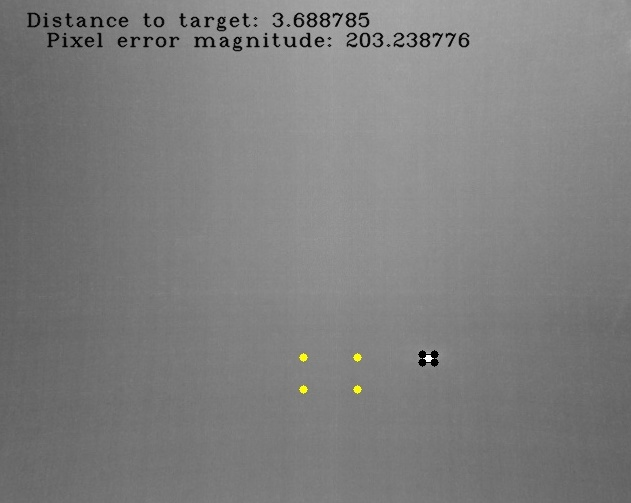
\includegraphics[width=8cm, height=7cm]{Images/initial.jpg}
% \caption{Initial view from thermal camera before starting visual servoing. Desired pixels in yellow and target pixels in black.}
% \label{initial}
% \end{figure}

% \begin{figure}
% \centering
% 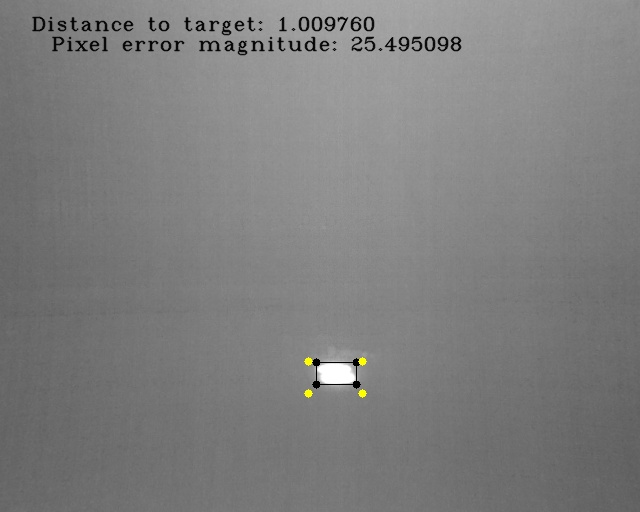
\includegraphics[width=8cm, height=7cm]{Images/final.jpg}
% \caption{Final view from thermal camera at the end of visual servoing. Desired pixels in yellow and target pixels in black.}
% \label{final}
% \end{figure}
\begin{figure}%[htbp]
    \begin{minipage}[t]{0.475\linewidth}
        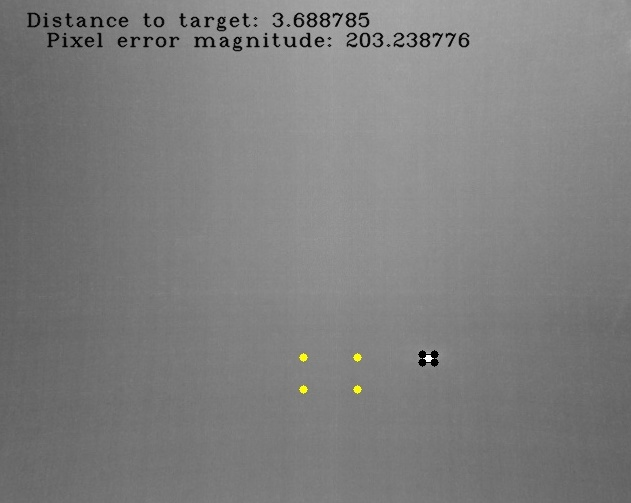
\includegraphics[width=\linewidth]{Images/initial.jpg}
        \caption{Initial view from thermal camera before starting visual servoing. Desired pixels in yellow and target pixels in black.}
        \label{initial}
    \end{minipage}%
        \hfill%
    \begin{minipage}[t]{0.475\linewidth}
        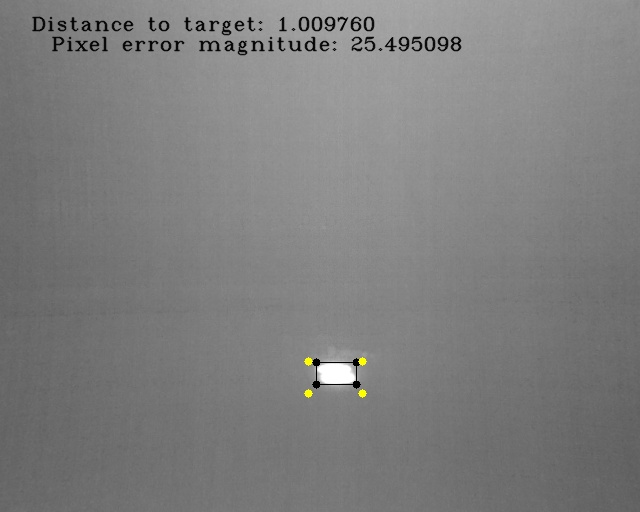
\includegraphics[width=\linewidth]{Images/final.jpg}
        \caption{Final view from thermal camera at the end of visual servoing. Desired pixels in yellow and target pixels in black.}
        \label{final}
    \end{minipage} 
\end{figure}

\begin{figure}
\centering
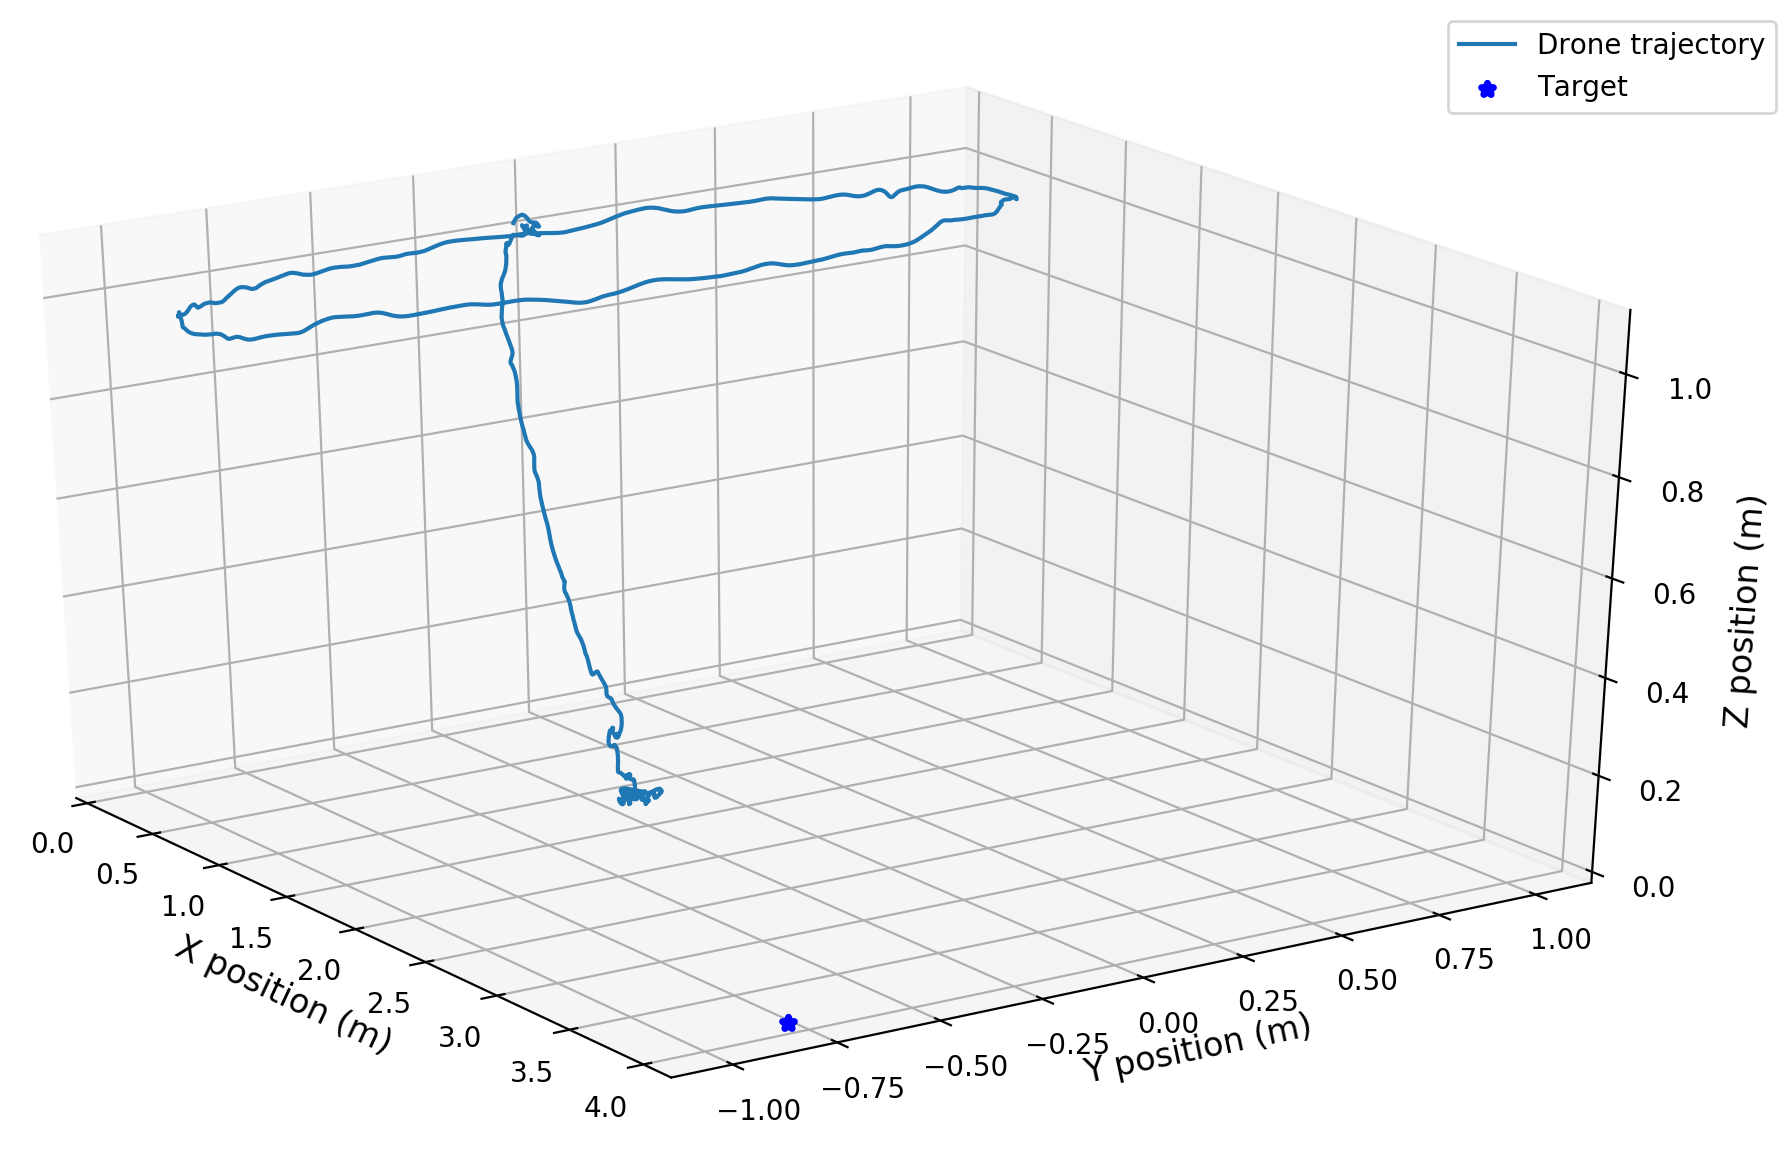
\includegraphics[width=8.5cm, height=7cm]{Images/3d_pos_traj.png}
\caption{Full drone position trajectory during the complete experiment.}
\label{full_drone_traj}
\end{figure}

\section{Conclusion}
In this paper, a solution architecture for landmine detection was presented, using a frontal and fixed thermal camera mounted on a drone quadrotor. Experiments were performed in a constrained environment, using Optitrack system to emulate the GPS measurements. In order to perform the visual servoing, depth estimation was needed, and our previous work on target position estimation helped us to get an accurate initial depth estimate for the IBVS algorithm. As can be seen from the results on Fig. \ref{pixel_error} and Fig.\ref{tgt_depth_est}, the initial estimation approaches to the real values, after stage 1 is completed. As the drone changes to stage 2, the estimation deviates slightly from the real values, due to the lack of variation on the azimuth and elevation angles at short distance from the target. 

In terms of IBVS, although the total pixel error is reduced significantly, as the drone gets closer to the target, the produced velocities from IBVS are too small to be perceived by the drone velocity controllers, results in a residual total error.

In the general perspective of this work, the proposed solution shows a feasible alternative for landmine detection, as long as a differences in temperature between the ground soil in the mine fields and the possible targets exist.

\bibliographystyle{IEEEtran}
\bibliography{IEEEfull,ibvs_drone}


\end{document}
